\documentclass[11pt]{scrartcl}
\usepackage[scale=1.5]{ccicons}
\usepackage[notextcomp]{kpfonts} 
\usepackage[margin=1.0in]{geometry}
\usepackage{amsthm,amssymb,amsmath}
\usepackage[]{graphicx}
\usepackage{subcaption}
\usepackage{enumitem}
\usepackage{bm}
\usepackage{tabu}
\usepackage{mathtools}
\usepackage{tikz}
\usepackage{tikz-3dplot}
\usepackage{xcolor}
\usepackage{colortbl}
\usepackage{wasysym}



\usepackage{color}
\definecolor{darkblue}{rgb}{0, 0, .6}
\definecolor{grey}{rgb}{.7, .7, .7}
\usepackage[breaklinks]{hyperref}
\hypersetup{
	colorlinks=true,
	linkcolor=darkblue,
	anchorcolor=darkblue,
	citecolor=darkblue,
	pagecolor=darkblue,
	urlcolor=darkblue,
	pdftitle={},
	pdfauthor={}
}
%\usepackage{fancyhdr}
%\thispagestyle{fancy}
%\lhead{Math 107}
%\chead{Lesson Plans}
%\rhead{Spring 2018}
%\lfoot{}%\scriptsize This work is licensed under the \href{http://creativecommons.org/licenses/by-sa/3.0/us/}{Creative Commons Attribution-Share Alike 3.0 License}.} 
%\cfoot{}
%%\rfoot{\ccbysa}
%\renewcommand{\headrulewidth}{.4pt}
%\renewcommand{\footrulewidth}{.4pt}

\theoremstyle{definition}
\newtheorem{theorem}{Theorem}
\newtheorem*{theorem*}{Theorem}
\newtheorem{acknowledgement}[theorem]{Acknowledgement}
\newtheorem{algorithm}[theorem]{Algorithm}
\newtheorem{axiom}[theorem]{Axiom}
\newtheorem{case}[theorem]{Case}
\newtheorem{claim}[theorem]{Claim}
\newtheorem*{claim*}{Claim}
\newtheorem{conclusion}[theorem]{Conclusion}
\newtheorem{condition}[theorem]{Condition}
\newtheorem{conjecture}[theorem]{Conjecture}
\newtheorem{corollary}[theorem]{Corollary}
\newtheorem{criterion}[theorem]{Criterion}
\newtheorem{definition}[theorem]{Definition}
\newtheorem{example}[theorem]{Example}
\newtheorem{exercise}[theorem]{Exercise}
\newtheorem{journal}[theorem]{Journal}
\newtheorem{lemma}[theorem]{Lemma}
\newtheorem{notation}[theorem]{Notation}
\newtheorem{problem}[theorem]{Problem}
\newtheorem*{problem*}{Problem}
\newtheorem{proposition}[theorem]{Proposition}
\newtheorem{remark}[theorem]{Remark}
%\newtheorem{solution}[theorem]{Solution}
\newtheorem{summary}[theorem]{Summary}
\newtheorem{skeleton}[theorem]{Skeleton Proof}
\newtheorem{activity}[theorem]{Activity}
\newtheorem{intuitivedef}[theorem]{Intuitive Definition}

\DeclareMathOperator{\spn}{span}
\DeclareMathOperator{\Char}{Characteristic}
\DeclareMathOperator{\Aut}{Aut}
\DeclareMathOperator{\stab}{Stab}
\DeclareMathOperator{\Stab}{Stab}
\DeclareMathOperator{\orb}{\mathcal{O}}
\DeclareMathOperator{\lcm}{lcm}
\DeclareMathOperator{\gl}{GL}
\DeclareMathOperator{\Ker}{Ker}
\DeclareMathOperator{\Z}{\mathbb{Z}}
\DeclareMathOperator{\C}{\mathbb{C}}
\DeclareMathOperator{\R}{\mathbb{R}}
\DeclareMathOperator{\N}{\mathbb{N}}
\DeclareMathOperator{\Q}{\mathbb{Q}}
\DeclareMathOperator{\A}{\mathbb{A}}
\DeclareMathOperator{\Gal}{Gal}
\DeclareMathOperator{\PS}{\mathcal{P}}
\DeclareMathOperator{\acc}{acc}


\newenvironment{solution}{\begin{proof}[Solution]}{\end{proof}}
\newcommand{\comment}[1]{%
  \text{\phantom{(#1)}} \tag{#1}
}


%Useful for cut and paste
%\begin{enumerate}[label=\rm{(\alph*)}]

\begin{document}

%%%%%%%%%%%%%%%%%% Day 1 %%%%%%%%%%%%%%%%%%%%%

%\section*{Day 1: Course Policy and Section 3.1}
%\subsection*{Introduction and Frequency Tables}
%\hangindent=1cm \hangafter=1
%As students come in have them sit at their tables and answer/do the following questions/tasks:
%\begin{enumerate}[leftmargin=!,labelindent=1.5cm,itemindent=-15pt]
%	\item What year are you? (i.e. Freshman, Sophomore, etc)
%	\item What is the first letter of your last name?
%	\item What is your favorite movie that you have seen in the past 12 months?
%	\item How many miles away is your home from Tucson (driving)?
%	\item How many hours do you estimate you spend on your phone per day?
%\end{enumerate}
%Tell students about myself: 
%\begin{enumerate}[leftmargin=!,labelindent=1.5cm,itemindent=-15pt]
%	\item I have been teaching for 4 years now
%	\item first letter of my last name is L
%	\item my favorite movie that I have seen in the past 12 months is Wonder
%	\item it is 259.7 miles from Tucson to my home in Flagstaff (grew up there)
%	\item I estimate that I spend 2 hours on my phone per day, mostly checking email, texting and playing words in an email word game with my family.
%\end{enumerate}
%
%\noindent
%Ask students how they think I should get to know them as there is only one of me and 53 of them! Have them share with me their ideas (i.e. Holding up whiteboards, clickers etc.) Luckily for us we can create something called a \underline{Frequency Table}. Let's do this now!\\
%
%\noindent
%Create a Frequency Table for class standing: 31 Freshman, 12 sophomores, 4 juniors, 6 seniors\\
%
%\noindent
%Verbally discuss (using our English skills) why this makes sense.
%
%\subsection*{Course Policy}
%Take a break and talk about this course a little bit. Emphasize important aspects of the Course Policy. Talk about how this is a class that has some math in it but the important part is to learn how to think. USE THIS AS A TImE TO SELL THE mETHOD THAT WE ARE GOING TO USE, not too much lecture mostly them doing things.
%
%\subsection*{Relative Frequency}
%I know that Dr. Gillette's math 107 class at 11 has a frequency chart that looks like this project his chart. Which class has more freshman relative to the overall population?\\
%
%\noindent
%Create relative frequency chart for our class, and display Andrew's. Which class has more freshman relative to the overall population? Which class has more freshman?\\
%
%\noindent
%Define relative frequency: 
%
%\subsection*{Categorical vs. Numerical Variables}
%Can we create a frequency table based on question 4 or 5 from the introduction questions?\\
%What is the difference between this question and question 1?\\
%
%\noindent
%Define Categorical Variable: is a variable that consists of names or labels of groups or individuals (like class standing, letter of your last name etc, things that we can easily sort into bins laundry example)\\
%
%\noindent
%Define Numerical Variable: is a variable that consists of measurable quantities to describe something (like miles from home, time spent on your phone)\\
%
%\noindent
%In your groups decide whether the following are categorical or numerical variables:
%\begin{enumerate}[leftmargin=!,labelindent=1.5cm,itemindent=-15pt]
%	\item The mode of transportation you take to class
%	\item The area code of your cell phone number
%	\item The number on the back of a UA basketball players jersey
%	\item The gas mileage of a car
%\end{enumerate}
%
%\subsection*{Frequency and Relative Frequency Bar Graphs}
%The following is the first initial of the last name of everyone in the class. Using this information create a frequency and relative frequency chart that represents this data.
%\begin{center}
%	\begin{tabular}{llllllllll}
%m & N & G & S & G & H & Q & T & G & R \\
%P & D & R & C & L & B & D & R & S & Z \\
%C & J & K & R & S & L & P & T & E & K \\
%m & C & m & P & P & D & m & C & m & T \\
%W & m & D & I & H & C & G & J & E & m \\
%R & Y & G &   &   &   &   &   &   &  
%\end{tabular}
%\end{center}
%
%\noindent
%Sometimes we want more than just a Frequency/Relative Frequency table to display the data. How can we take this data and turn it into something that visually displays the information we want?\\
%
%\noindent
%Create the Frequency Bar Graph with the students modeling good graphing behaviors and have them try the relative frequency bar graph on their own. Show them both in Excel and talk about the only difference between the two is the y-axis


%%%%%%%%%%%%%%%%%% Day 2 %%%%%%%%%%%%%%%%%%%%%

%\section*{Day 2: Section 3.1 (End) and Section 3.2}
%\subsection*{Warm-Up/Intro Activity ~20-25 minutes} 
%	Recall last class we created a frequency and relative frequency table for the class standing of the students in our class. It looked something like this:\\
%	\begin{center}
%	\begin{tabular}{l|l|l}
%		
%		          & Frequency & Relative Frequency \\ \hline
%		Freshman  & 33        & 0.600              \\ \hline
%		Sophomore & 10        & 0.182              \\ \hline
%		Junior    & 4         & 0.073              \\ \hline
%		Senior    & 8         & 0.145              \\ \hline
%		Total     & 55        & 1                  \\ 
%	\end{tabular}	
%	\end{center}
%	Use this to answer the following questions on the white board at your table as a group.
%	
%	\begin{enumerate}
%		\item Draw a bar graph that represents the frequency column.
%		\item Draw a bar graph that represents the relative frequency column.
%		\item What differences are there between the two graphs you created?
%		\item How many students are freshman OR sophomores?
%		\item What proportion of students are freshman AND seniors?
%	\end{enumerate}
%	
%	\noindent
%	For this problem, no clickers have tables volunteer the information. Show bar graphs completed in Excel. At the end discuss how we would make a pie chart from the given information. Show in Excel.
%	
%\subsection*{Two-way tables ~15-20 min}
%	Sometimes we have more information than just one categorical variable. At the beginning of class we collected your information about your gender and favorite tv show from the top 3 shows of the year. The responses are posted in an Excel document in D2L. 
%	
%	\noindent
%	\textcolor{red} {Have Ryan put the data into Excel and post as an announcement}\\
%	
%	\noindent
%	As a group create a table on your whiteboard that displays the information that was just posted in the announcement in D2L. \textcolor{red}{make announcement in D2L}\\
%	
%	\noindent
%	This is called a two-way table, and consists of two categorical variables.\\ 
%	
%	\newpage
%\subsection*{AND and OR Proportions ~20-25 min}
%	\noindent
%	Let's study this one now.\\
%	
%	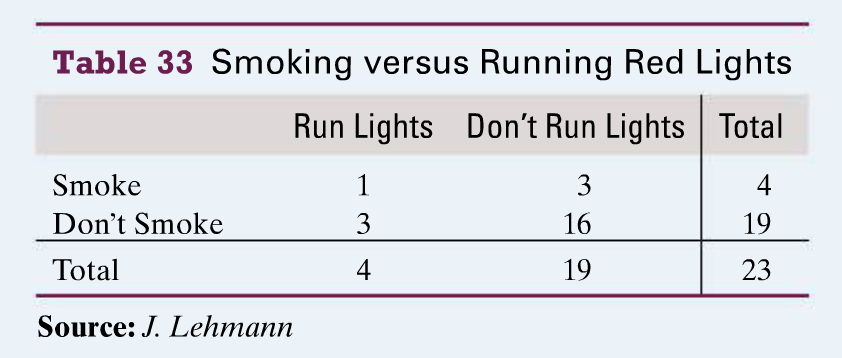
\includegraphics{twoway}
%	
%	Answer the following questions about the data presented above:
%	\begin{enumerate}
%		\item How many people don't smoke?
%		\item How many people run red lights?
%		\item What proportion of people smoke AND don't run red lights?
%		\item What proportion of people don't smoke OR run lights?	
%	\end{enumerate}
%	
%\subsection*{Summary of what we know so far ~5min}
%	Two different types of variables are:\\
%	\hspace{2cm} \underline{\hspace{2cm}} which describes data that is \underline{\hspace{2cm}}\\
%	\underline{\hspace{2cm}} which describes data that is \underline{\hspace{2cm}}.\\
%	
%	\noindent
%	We use the following things to describe categorical data:
%	\begin{itemize}
%		\item \underline{\hspace{5cm}}
%		\item \underline{\hspace{5cm}}
%		\item \underline{\hspace{5cm}}
%		\item \underline{\hspace{5cm}}
%		\item \underline{\hspace{5cm}}
%		\item \underline{\hspace{5cm}}
%	\end{itemize}
%
%
%	\subsection*{Course Policy Quiz on Clickers ~10 min}

%%%%%%%%%%%%%%%%%% Day 3 %%%%%%%%%%%%%%%%%%%%%
%\section*{Day 3: Section 3.3}
%
%\subsection*{Warm-Up/Intro Activity 20-25 minutes}
%Part 1: The following is a table that compares class standing to types of body art from a undergraduate students at a certain university. 
%
%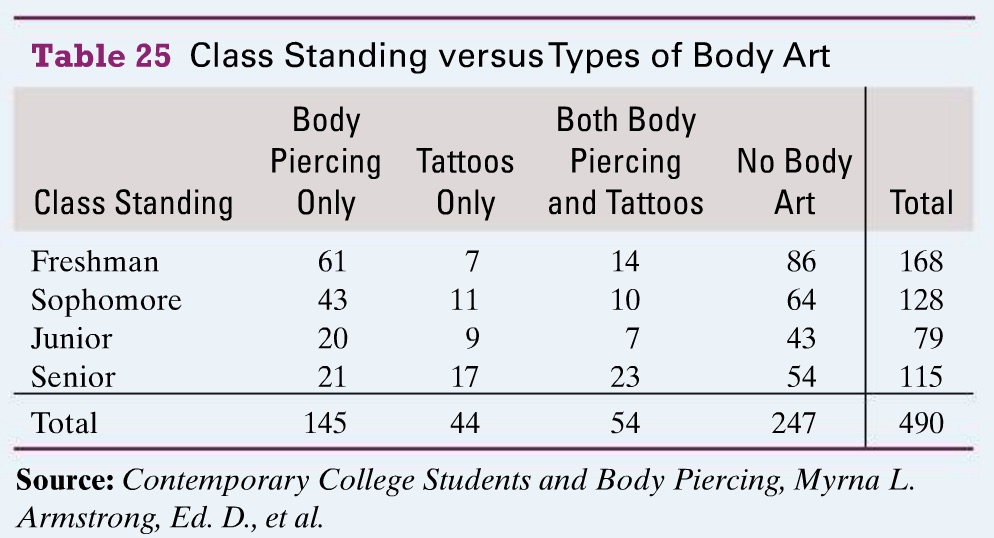
\includegraphics[scale=0.45]{bodyartclassstanding}
%
%\noindent
%Use it to answer these questions:
%\begin{enumerate}
%	\item How many students have Body Piercings Only AND are Sophomores?
%	\item What proportion of students have no body art AND Seniors?
%	\item How many students are Sophomores OR Tattoos Only?
%	\item What proportion of students have Both Body Piercing and Tattoos OR are Juniors?
%\end{enumerate}
%
%\noindent
%Part 2: Consider the following numerical variables and decide what types of numbers are used to measure them (whole numbers, fractions, etc)
%\begin{enumerate}
%	\item Age
%	\item Number of times a person went out last year
%	\item Gas mileage of a car
%	\item Height
%	\item Number of strings on a musical instrument
%	\item Clothing sizes
%\end{enumerate}
%
%\noindent
%Define the following:\\
%\textbf{Continuous Variable:} A variable that can take on any value between two variables.\\
%\textbf{Discrete Variable:} A variable that has gaps between successive, possible values.\\
%
%\noindent
%\textbf{Note:} It is important to consider possible values before rounding. Go back through and determine continuous or discrete.
%
%
%
%\newpage
%\subsection*{Dot Plots}
%The following is a dotplot that represents the asking price for certain four bedroom houses in thousands of dollars in Arkon, Ohio:
%\begin{center}
%	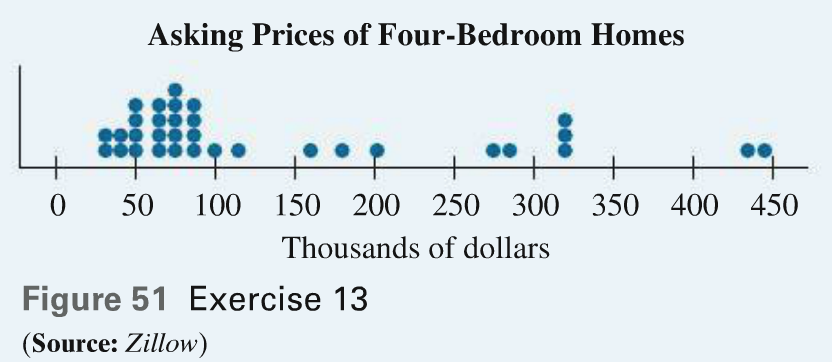
\includegraphics{dotplot}
%\end{center}
%
%\noindent
%Answer the following questions about this data:
%\begin{enumerate}
%	\item What is the frequency of the number of four bedroom houses that sold for \$75,000?
%	\item Are any dates much larger or smaller than the others? Why do you think this might be?
%	\item What house price is larger than or equal to 20\% of all other states? $\ldots$ 50\% of all other states? $\ldots$ 80\% of all other states?
%\end{enumerate}
%
%\noindent
%Define the following:\\
%\textbf{Percentile:} The $k-$th percentile is a number (possibly not in the original data) at which $k\%$ of the data fall below that number.
%
%\subsection*{Stemplots}
%Using the same data as the previous example work with your group to answer the following questions:
%
%	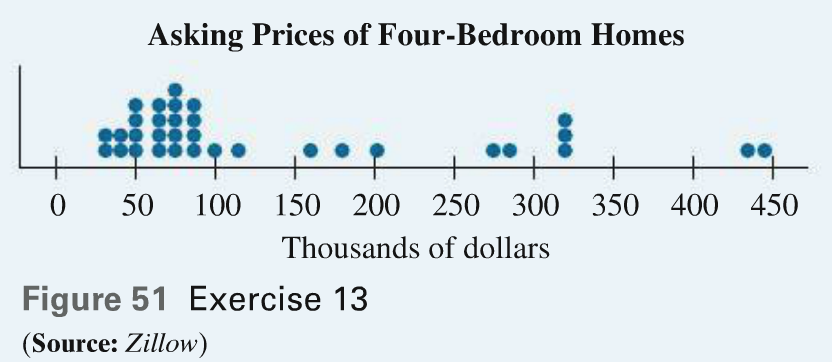
\includegraphics{dotplot}
%
%
%\begin{enumerate}
%	\item make a stemplot (sometimes known as a stem and leaf) plot that represents this data.
%	\item What value represents the 25th percentile? $\ldots$ the 60th percentile? $\ldots$ the 90th percentile?
%\end{enumerate}
%
%\subsection*{Excel and Gradescope}

%%%%%%%%%%%%%% Day 4: Section 3.4 %%%%%%%%%%%%%%%
%\section*{Day 4: Section 3.4}
%\subsection*{Warm-Up/Intro Activity}
%Using the same data as the previous example work with your group to answer the following questions:
%
%	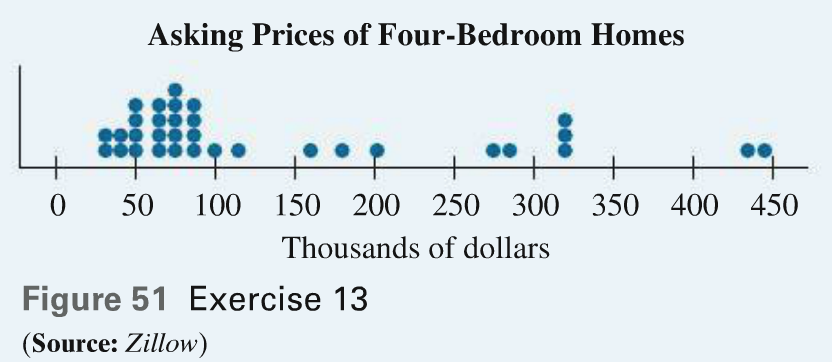
\includegraphics[scale=0.25]{dotplot}
%
%
%\begin{enumerate}
%	\item make a stemplot (sometimes known as a stem and leaf) plot that represents this data.
%	\item What value represents the 25th percentile? $\ldots$ the 60th percentile? $\ldots$ the 90th percentile?
%\end{enumerate}
%
%\subsection*{Intro Example}
%With larger data sets creating a dot plot or stem plot is cumbersome and not realistic as it would get to big. To combat this we can create ``classes" which allow us to group the data in a realistic way to create a ``bar graph."\\
%
%\noindent
%Using the data from the data from the intro activity create a frequency table that has a lower class limit of 25 and a class width of 50. Here we are working with thousands of dollars.
%
%\subsection*{Definitions and Examples}
%Unimodal, Bimodal, and multimodal
%\begin{figure}[h!]
%\centering
%\begin{subfigure}{.5\textwidth}
%  \centering
%  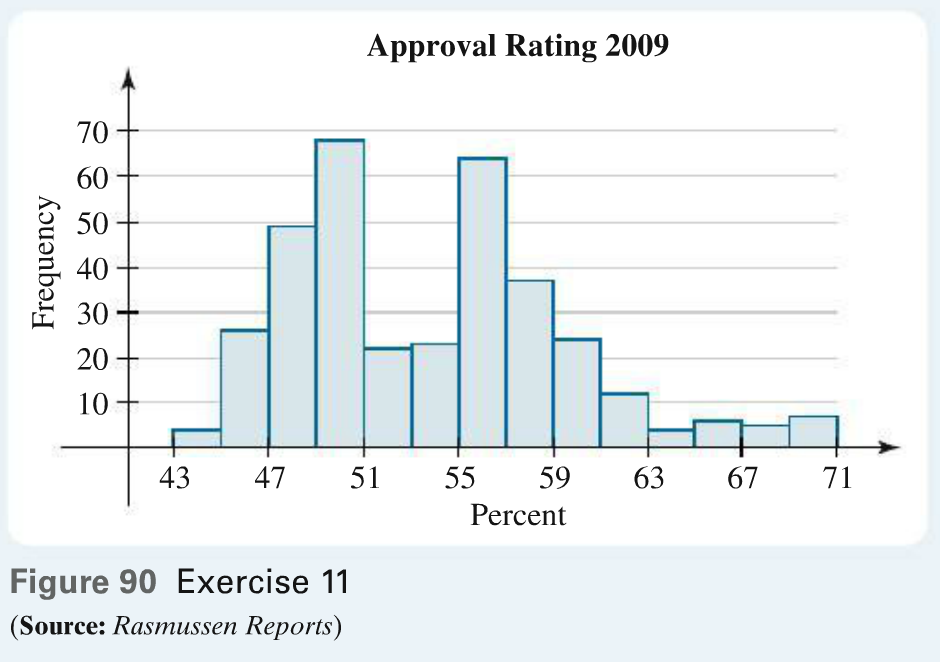
\includegraphics[scale=0.45]{Bimodal}
%\end{subfigure}%	
%\begin{subfigure}{.5\textwidth}
%  \centering
%  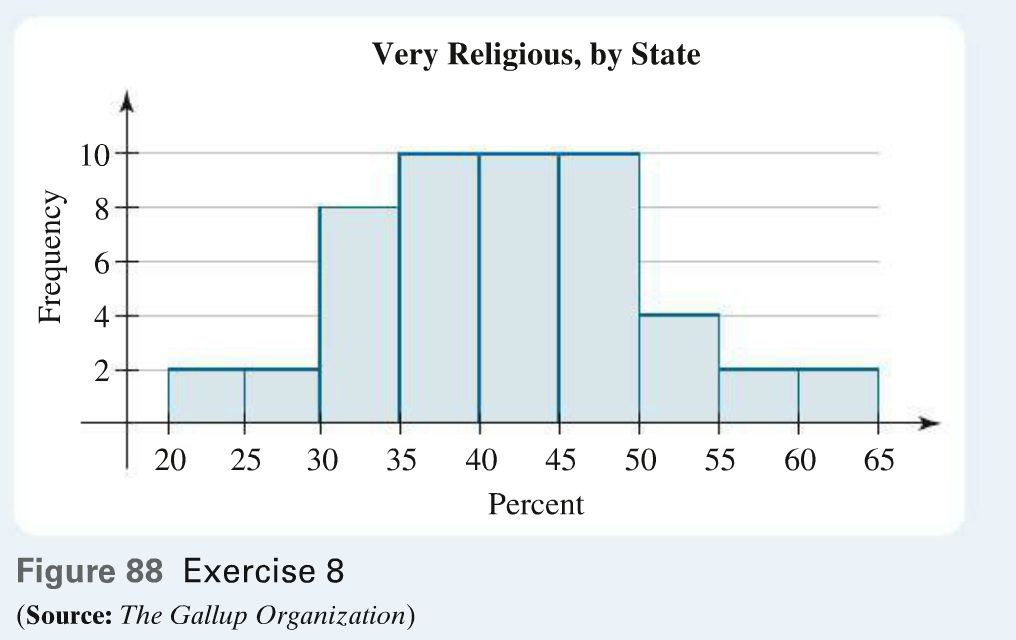
\includegraphics[scale=0.45]{Symmetric}
%\end{subfigure}
%\end{figure}
%
%\noindent
%Left-Skewed vs Right Skewed vs Symmetric
%\begin{figure}[h!]
%
%\begin{subfigure}{.5\textwidth}
%
%  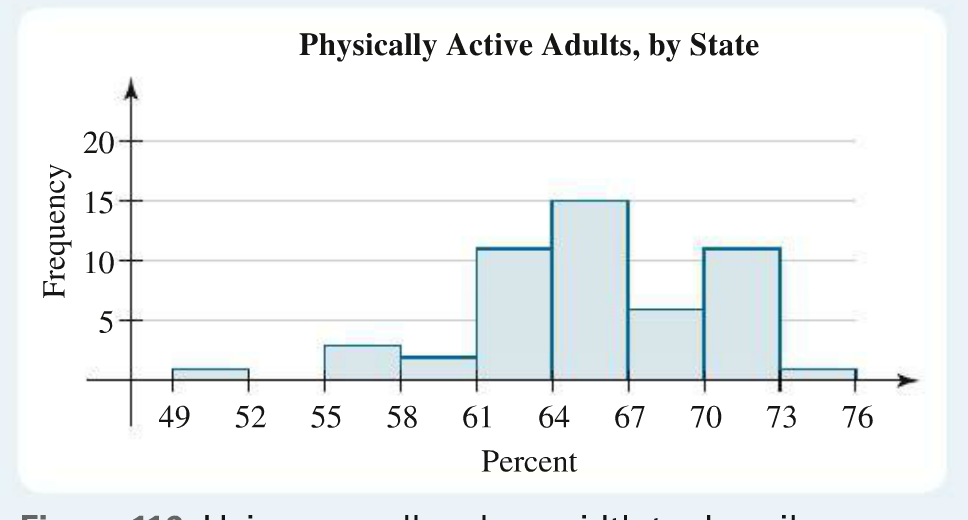
\includegraphics[scale=0.45]{Left_Skewed}
%\end{subfigure}%	
%\begin{subfigure}{.5\textwidth}
%
%  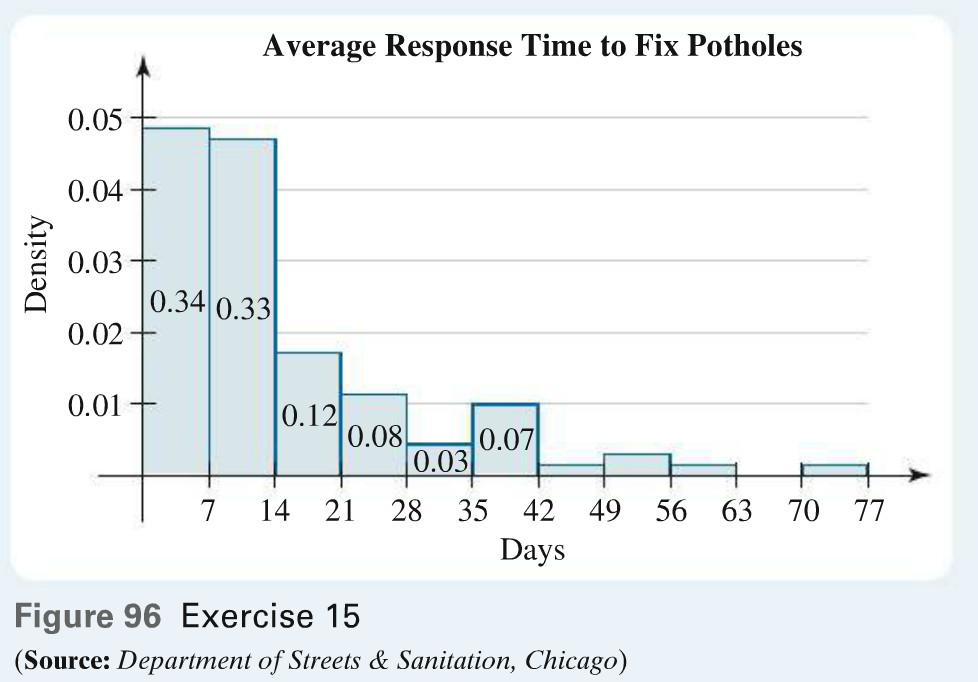
\includegraphics[scale=0.45]{Right_Skewed}
%\end{subfigure}
%\end{figure}
%
%\subsection*{Example}
%Scientists visited 30 sites along the Colorado River and counted the number of seedlings of Cottonwood trees. The following is their counts:
%\begin{center}
%	\begin{tabular}{llllll}
%48  & 49  & 52  & 54  & 54  & 57  \\
%61  & 63  & 67  & 67  & 69  & 70  \\
%70  & 72  & 73  & 73  & 76  & 79  \\
%79  & 83  & 85  & 87  & 96  & 98  \\
%103 & 105 & 108 & 112 & 138 & 139
%\end{tabular}
%\end{center}
%
%\noindent
%\textbf{Even Numbered Tables:} Construct a histogram using classes that start at 48 and have a class width of 19.\\
%
%\noindent
%\textbf{Odd Numbered Tables:} Construct a histogram using classes that start at 48 and have a class width of 10.
%
%\noindent
%Some questions to answer after they are done:
%\begin{enumerate}
%	\item Describe the shape of the histogram.
%	\item Are there any outliers?
%	\item What is the 25th percentile? 50 percentile? 75th percentile?
%	\item What percentile does the observation 85 correspond to? What does this mean?
%\end{enumerate}
%
%\subsection*{Clicker Questions}
%Ask the following questions throughout class:
%\begin{enumerate}
%	\item Are you here on time?
%	\item What value represents the 50th percentile?
%	\item If you are creating a histogram with a class/count table that starts at 12 and has a class width of 27, what is the upper bound of the first class?
%	\item Looking at the following histogram describe its shape (unimodal, bimodal, multimodal, left skewed, right skewed, symmetric). \begin{center} 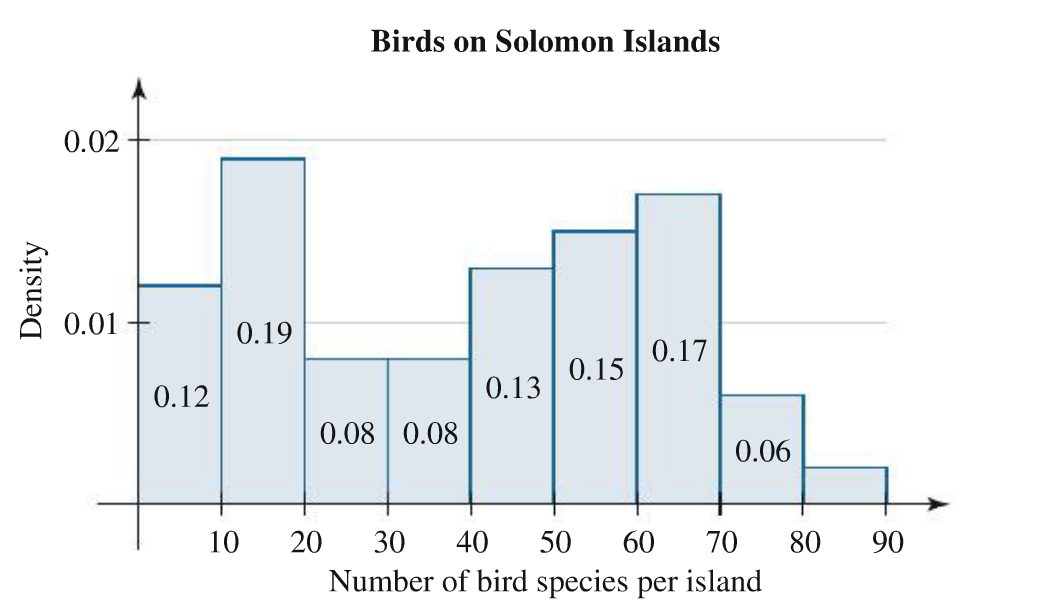
\includegraphics[scale=0.5]{histogramclicker} \end{center}
%\end{enumerate}

%%%%%%%%%%%%%%%%%%% Day 5: Section 3.4 & Quiz %%%%%%%%%%%%%%%%%%%

%\section*{Day 5: Section 3.4 and Quiz 1}
%\subsection*{Warm-Up/Intro Activity}
%Copy the following into your notes and fill in the blanks.\\
%
%\noindent
%A \underline{\hspace{5cm}} consists of names  or labels of groups of individuals.\bigskip\\
%
%\noindent
%A \underline{\hspace{5cm}} consists of measurable quantities that describe individuals.\bigskip\\
%
%\noindent
%We use a \underline{\hspace{5cm}} or a \underline{\hspace{5cm}} to display categorical variables in a readable format where the \underline{\hspace{5cm}} is the number of observations in that category and the \textbf{relative frequency} is calculated by \underline{\hspace{5cm}} and they sum to \underline{\hspace{5cm}}.\bigskip\\
%
%\noindent
%The following is a list of displays for categorical data:
%\begin{itemize}
%	\item 
%	\item
%	\item
%	\item
%	\item
%\end{itemize}
%
%\noindent
%When we use the word \textbf{AND} we are including observations that satisfy \underline{\hspace{5cm}} (2 words). Using the word \textbf{OR} we are including observations that satisfy \underline{\hspace{5cm}} (3 words).\bigskip \\
%
%\noindent
%A \textbf{discrete variable} is a \underline{\hspace{5cm}} variable that has \underline{\hspace{5cm}} between successive, possible values.\bigskip\\
%
%\noindent
%A \textbf{continuous variable} is a \underline{\hspace{5cm}} variable that can take on \underline{\hspace{5cm}} between two possible values.\bigskip\\
%
%\noindent
%The following is a list of displays for numerical data:
%\begin{itemize}
%	\item 
%	\item
%	\item
%	\item
%\end{itemize}
%\bigskip
%
%\noindent
%The \underline{\hspace{5cm}} of some data is a value (not necessarily a data value) that is bigger than or equal to k\% of the observations.\bigskip \\
%
%\noindent
%Draw a picture of a histogram that is:
%\begin{itemize}
%	\item unimodal
%	\item bimodal
%	\item multimodal
%	\item right skewed
%	\item left skewed
%\end{itemize}
%
%\subsection*{Practice constructing histograms and with percentiles}
%The following data are the numbers of endangered species in randomly selected African questions.\\
%\begin{center}
%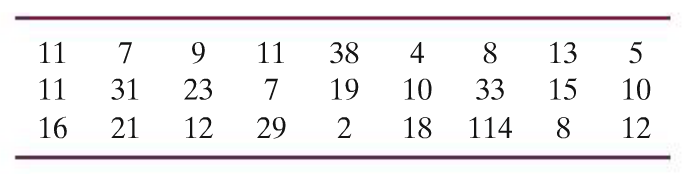
\includegraphics{africadata}
%\end{center}
%Use this data to answer the following questions:
%\begin{enumerate}
%	\item Construct a histogram that has a class width of 19 and starts at 2.
%	\item Describe the shape of the histogram.
%	\item Are there any outliers?
%	\item What class does the 50th percentile fall into? In relation to the histogram, where is the 50th percentile located?
%\end{enumerate}
%
%\begin{center}
%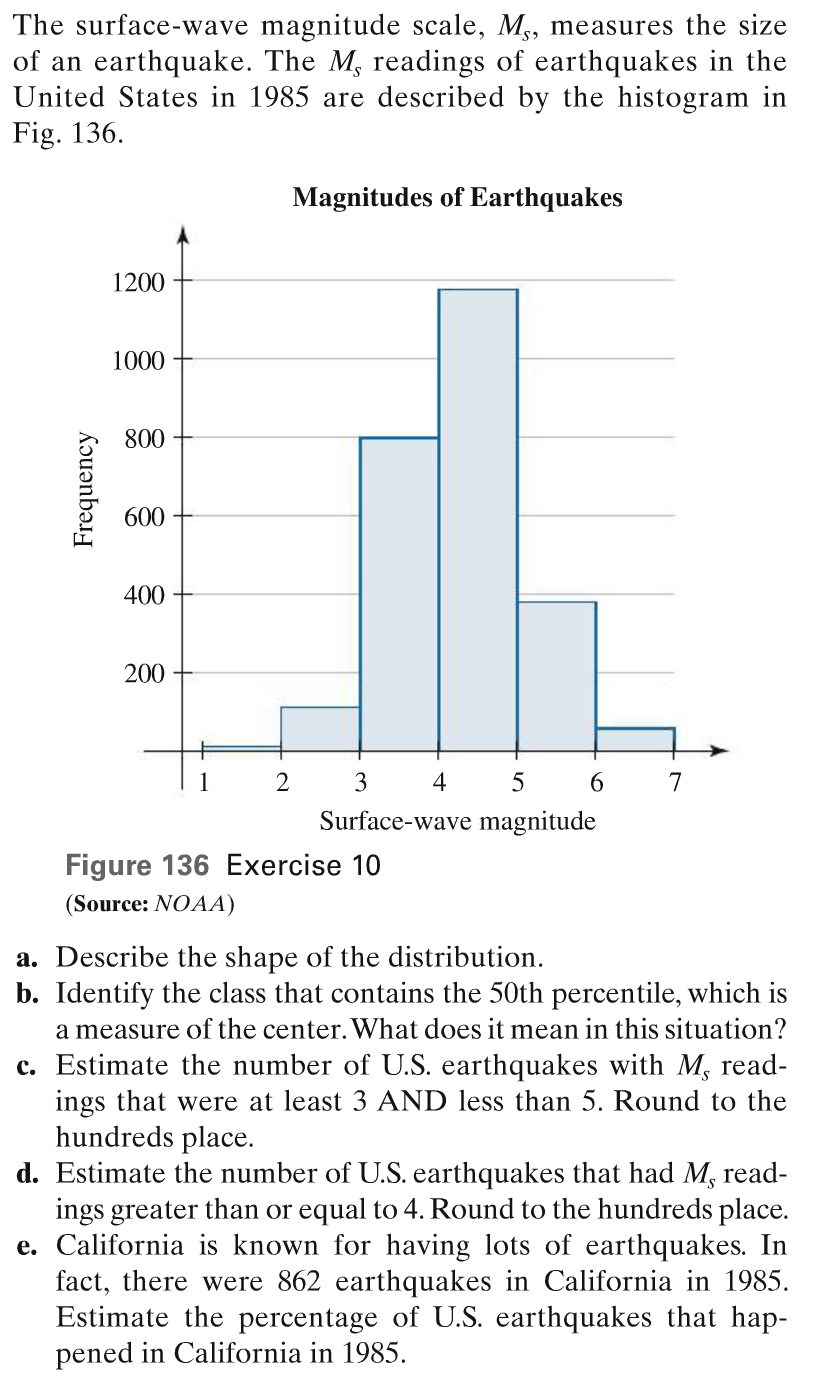
\includegraphics[scale=0.45]{Histogrampractice}	
%\end{center}

%%%%%%%%%%%%%%%%%%% Day 6: Section 4.1 %%%%%%%%%%%%%%%%%%%

%\section*{Section 4.1}
%\subsection*{Warm-Up/Intro Activity ($\sim$ 30min)}
%The following is the amount of money that Jos\'{e} spent on lunch the past 12 days at school.
%\begin{center}
%	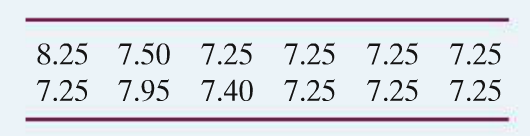
\includegraphics{LunchPrices}
%\end{center}
%Use this information to answer the following questions:
%\begin{enumerate}
%	\item Calculate the following in regards to the data:
%		\begin{itemize}
%			\item mean
%			\item median
%			\item mode
%		\end{itemize}
%	\item Considering the above numbers, write a sentence that Jos\'{e} could use to persuade his parents that he isn't spending too much on lunch.
%	\item Now consider the perspective of Jos\'{e}'s parents, write a sentence that they could use to persuade Jos\'{e} he is spending too much on lunch.
%	\item Suppose instead on day 11 Jos\'{e} spent \$12.25 and on day 12 he spent \$10.50. Repeat the above exercises.
%\end{enumerate}
%
%\noindent
%Students will complete this exercise at their tables with assistance from the instructors/TAs in the room. \\
%
%\noindent
%If a group finishes early the group should be prompted to think about the second scenario and what we would call the added prices (outliers). Then they should be prompted to think about how outliers affect the mean and the median.
%
%\subsection*{Definitions}
%Define \textbf{mean}-(the sum of the observations divided by the number of observations), \textbf{median}-(the median is the 50th percentile, the middle of the data), and \textbf{mode}-(the observation with the greatest frequency)
%
%\subsection*{Examples of how mean/median work with regards to outliers and calculators}
%Use this data to answer the following questions:
%\begin{center}
%	\includegraphics{meanmedian}	
%\end{center}
%
%\begin{itemize}
%	\item For this activity you need your graphing calculator out.
%	\item Agree on one persons computer to use for this activity and open the mymathLab textbook to page A-2 to find directions how to input data into a list.
%	\item Once the data is input into the list go to page A-4 to find directions on how to compute mean, median and other standard deviations of the data.
%\end{itemize}
%
%\begin{enumerate}
%	\item Record the mean ($\overline{x}$) and median (med) on one of the white boards at your table. Create a histogram that represents this data with a class width of 2 that has a lower class limit of 10. (Remember if a data value falls on the border of a class we include it in the class it is the upper limit for)
%	\item Complete the following activity:
%		\begin{itemize}
%			\item \textbf{EVEN Tables:} Remove the top 3 values from the original data and replace them with the values 40, 40, 41
%			\item \textbf{ODD Tables:} Remove the bottom 3 values from the original data and replace them with the values 2, 2, 4.
%		\end{itemize}
%	\item Compare your findings with a table that is the opposite of yours and write a sentence with your table mates about how outliers affect the mean and median.	
%\end{enumerate}
%
%\noindent
%Discussion regarding the outliers affect on mean and median. The mean is sensitive to outliers, the median is resistant to outliers.
%
%\subsection*{Skewness and mean/median}
%\begin{figure}[h!]
%\centering
%\begin{subfigure}{.5\textwidth}
%  \centering
%  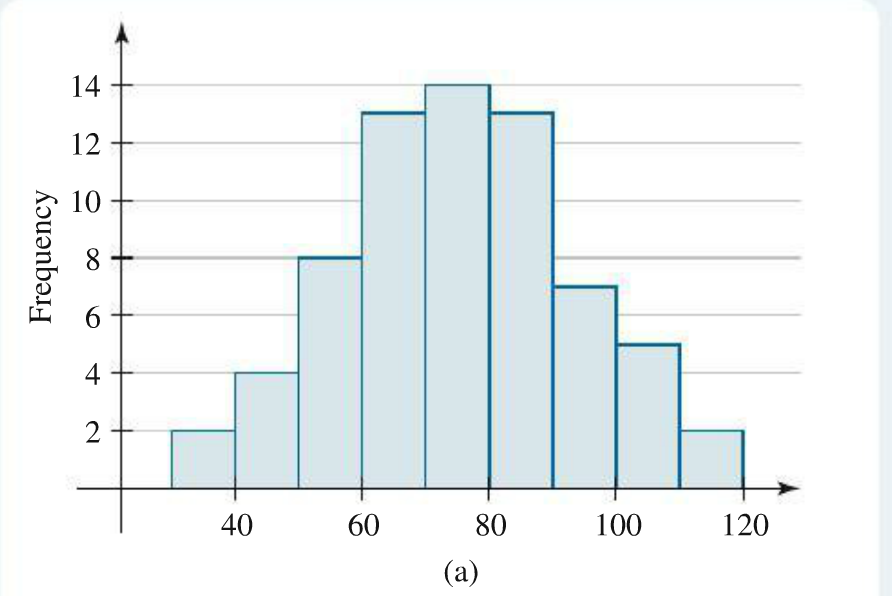
\includegraphics[scale=0.45]{Symmetric4}
%\end{subfigure}%	
%\begin{subfigure}{.5\textwidth}
%  \centering
%  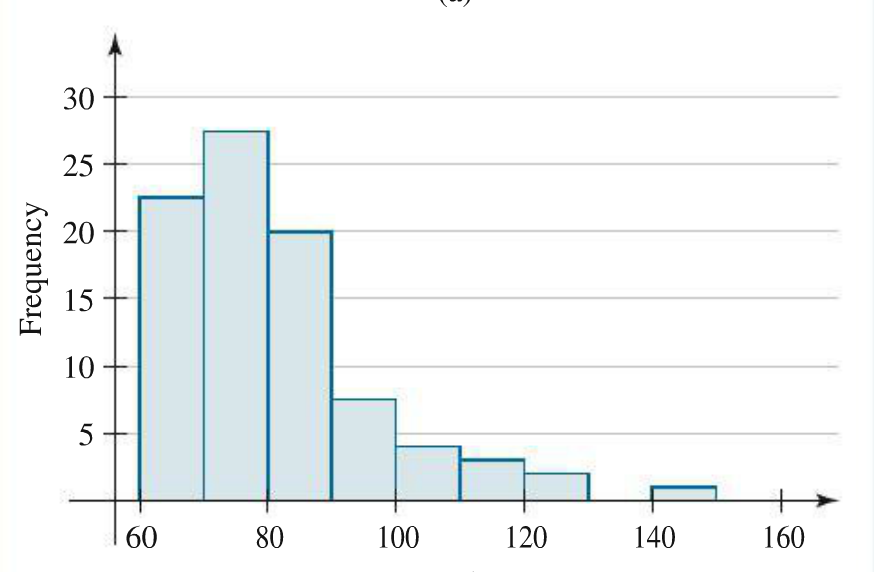
\includegraphics[scale=0.45]{RightSkewed4}
%\end{subfigure}
%\end{figure}
%
%\begin{center}
%	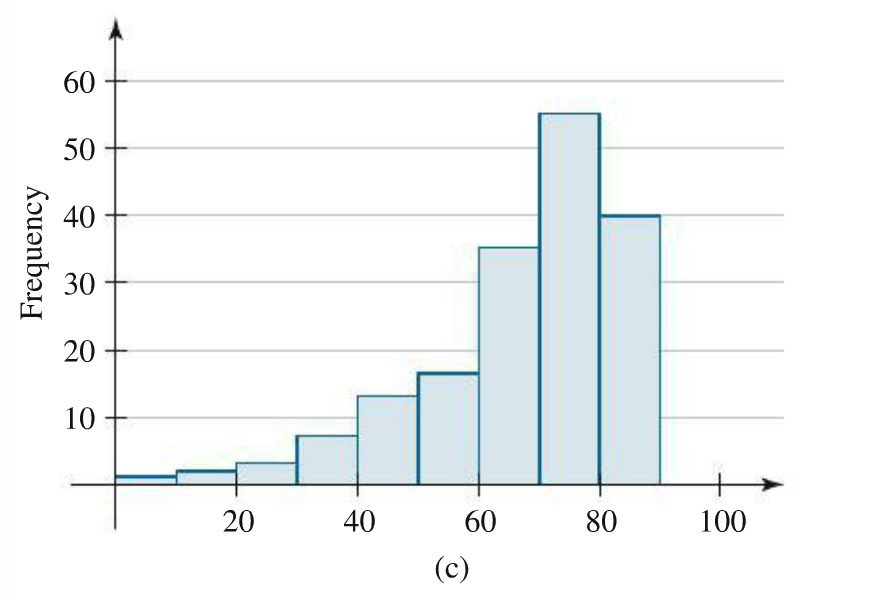
\includegraphics[scale=0.45]{LeftSkewed4}
%\end{center}
%
%\noindent
%Use the figures above to compare the mean and median for each set of data:\\
%
%\noindent
%Based on class discussion for each figure state whether the mean is equal to the median, the mean is less than the median or the mean is lower than the median.

%%%%%%%%%%%%%%%%%%% Day 6: Section 4.2 %%%%%%%%%%%%%%%%%%%

%\section*{Section 4.2}
%\subsection*{Warm-Up/Intro Activity}
%Consider the following 3 data sets:
%\[ A=\{7,9,10,11,13\} \hspace{3cm} B=\{10,10,10,10,10\} \hspace{3cm} C=\{1,1,10,19,19\} \]
%
%\noindent
%Calculate the mean and median for these three sets and record them on your whiteboard.\\
%
%\noindent
%The point of this activity is so that students see that measures of center aren't sufficient to describe data with and to lead to a discussion in regards to measures of spread (range/standard deviation). As a class we will calculate the standard deviation (using calculators) /range for each set and then discuss what this gives us a measure of.
%
%\subsection*{Practice with Standard Deviation/Range}
%The following data is the number of calories in one slice ($\frac{1}{8}$th of a 14" Pizza) at Pizza Hut:
%
%\begin{center}
%	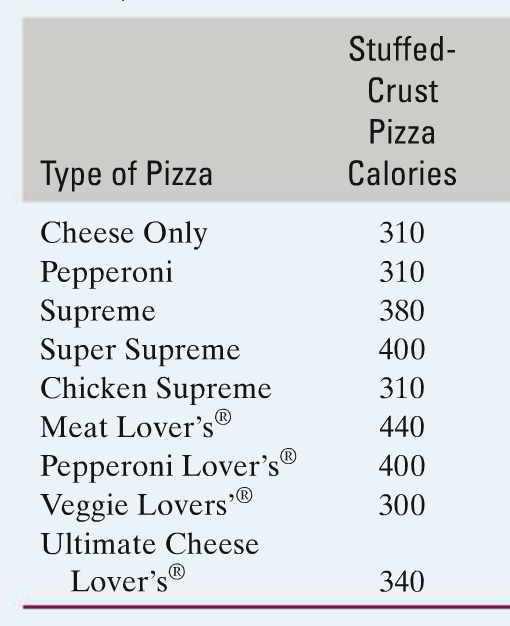
\includegraphics[scale=0.5]{StdDev}
%\end{center}
%
%\noindent
%Calculate the mean and standard deviation of the number of calories in one slice of pizza from Pizza Hut. Explain in context of the problem what this means.
%
%\subsection*{Properties of Standard Deviation/Range Exploration}
%Recall one of the data sets from the beginning of class:
%\[A=\{7,9,10,11,13\} \]
%
%\noindent
%We found the following measurements regarding it:
%\begin{itemize}
%	\item $\overline{x}=10$
%	\item $m=10$
%	\item $R=6$
%	\item $s=2.236$
%\end{itemize}
%
%\noindent
%Answer the following questions:
%\begin{enumerate}
%	\item Add 5 to each of the data values in the set and calculate the mean, median, standard deviation and range for the new set of values. Write a sentence that explains how the new values compare to the original values.
%	\item multiply each value by 5 and calculate the mean, median, standard deviation, and range for the new set of values. Write a sentence that explains how the new values compare to the original values.
%	\item Using what you found in the Problem 1 and 2 to write a sentence that generalizes your findings.
%\end{enumerate}
%
%\subsection*{The Empirical Rule}
%Consider the following data set:
%
%\begin{center}
%	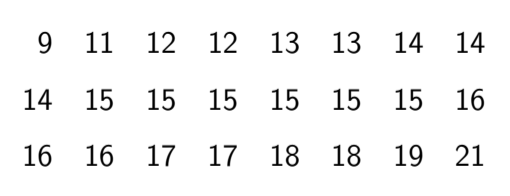
\includegraphics{EmpiricalRule}
%\end{center}
%
%Use it to answer the following questions:
%\begin{enumerate}
%	\item Calculate the mean and standard deviation for the given data.
%	\item Compute $\overline{x}-s$ and $\overline{x}+s$. Write a sentence that explains the computation you just completed.
%	\item How many observations lie within the values you computed above? What percentage of the overall observations is this?
%	\item Find the percentage of observations that lie within the values of $\overline{x}-2s$ and $\overline{x}+2s$.
%	\item Find the percentage of observations that lie with the values of $\overline{x}-3s$ and $\overline{x}+3s$.
%\end{enumerate}
%
%\vspace{1cm}
%
%\noindent
%\textbf{Empirical Rule:} If a distribution is unimodal and symmetric, approximately: 
%\begin{itemize}
%	\item 68\% of observations lie within 1 standard deviation of the mean ($\overline{x}-s$ to $\overline{x}+s$)
%	\item 95\% of observations lie within 2 standard deviations of the mean ($\overline{x}-2s$ to $\overline{x}+2s$)
%	\item 99.7\% of observations lie within 3 standard deviations of the mean ($\overline{x}-3s$ to $\overline{x}+3s$)
%\end{itemize}
%
%\subsection*{Deciding when to use mean/Standard Deviation or median/Range}
%Consider the following histograms:
%\begin{figure}[h!]
%\centering
%\begin{subfigure}{.5\textwidth}
%  \centering
%  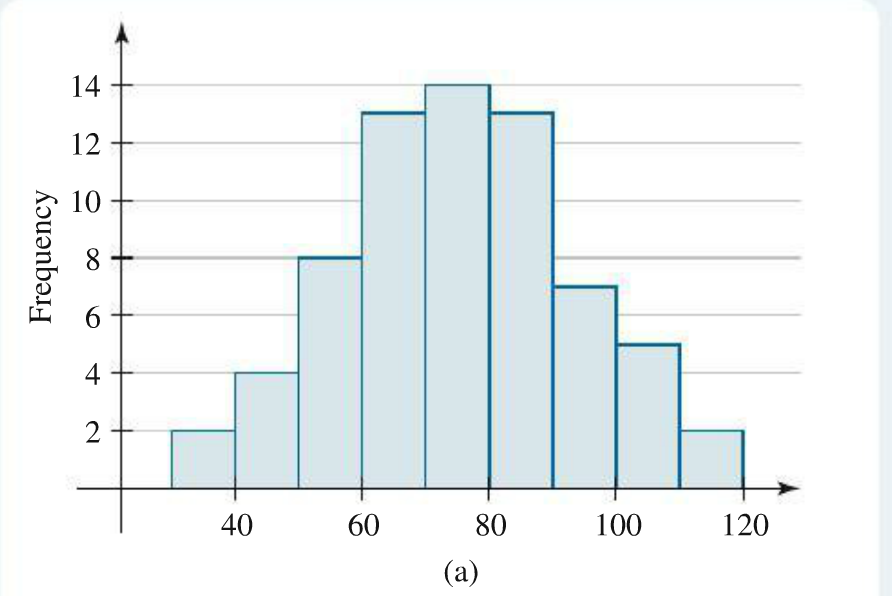
\includegraphics[scale=0.45]{Symmetric4}
%\end{subfigure}%	
%\begin{subfigure}{.5\textwidth}
%  \centering
%  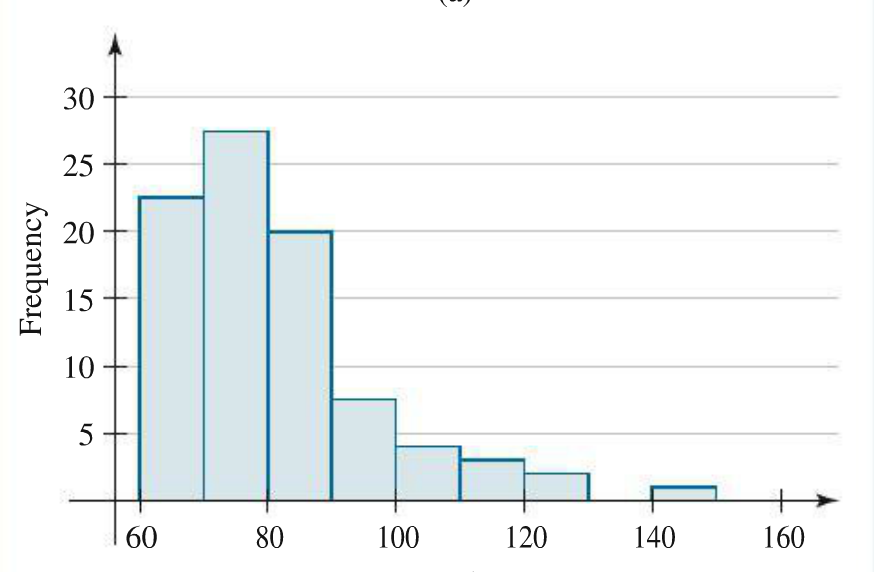
\includegraphics[scale=0.45]{RightSkewed4}
%\end{subfigure}
%\end{figure}
%
%\begin{center}
%	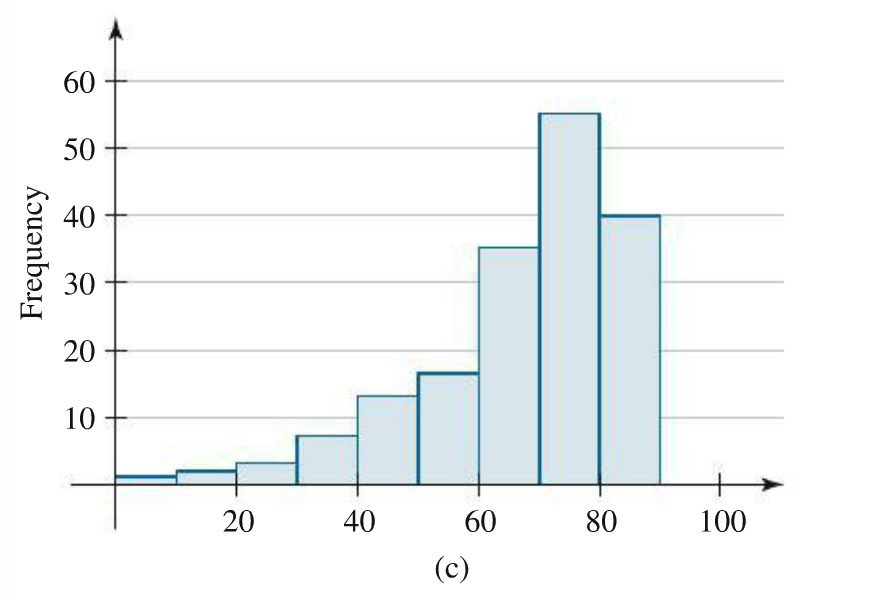
\includegraphics[scale=0.45]{LeftSkewed4}
%\end{center}
%
%\noindent
%As tables spend 30 seconds to decide which measure of center you would use to find the center of the data and why. Then discuss as a class which measure of spread. Write down somewhere on the page that mean and standard deviation go together with unimodal, symmetric data typically and median and range are used when data is skewed.
%
%\subsection*{Histogram matching Activity}
%This will be done as a clicker activity at the end of the class period. The students will work on the first one together and I will project the data in real time about what they chose for the question. After all students have submitted their answer, we will discuss as a class (remembering where the center of the data is and how we can tell what the standard deviation is). Once this is completed, the students will then answer the last questions regarding this on the clickers to see where we are at with the concepts presented in class.
%
%\begin{figure}[h!]
%\centering
%\begin{subfigure}{.5\textwidth}
%  \centering
%  \includegraphics[scale=0.45]{measureofCSHistograms}
%\end{subfigure}%	
%\begin{subfigure}{.5\textwidth}
%  \centering
%  \includegraphics[scale=0.45]{measureofCSHistograms2}
%\end{subfigure}
%\end{figure}
%
%\begin{itemize}
%	\item $\overline{x}= 40$, $s=2.5$
%	\item $\overline{x}= 40$, $s=12.4$
%	\item $m=70$, $R=7.6$
%	\item $m=70$, $R=38$
%\end{itemize}


%%%%%%%%%%%%%%%%%%% Day 8: Section 4.3 %%%%%%%%%%%%%%%%%%%

%\section*{Section 4.3}
%\subsection*{Warm-Up}
%Recall one of the data sets from last Thursday's class:
%\[A=\{7,9,10,11,13\} \]
%
%\noindent
%We found the following measurements regarding it:
%\begin{itemize}
%	\item $\overline{x}=10$
%	\item $m=10$
%	\item $R=6$
%	\item $s=2.236$
%\end{itemize}
%
%\noindent
%Answer the following questions:
%\begin{enumerate}
%	\item Add 5 to each of the data values in the set and calculate the mean, median, standard deviation and range for the new set of values. Write a sentence that explains how the new values compare to the original values.
%	\item multiply each value by 5 and calculate the mean, median, standard deviation, and range for the new set of values. Write a sentence that explains how the new values compare to the original values.
%	\item Using what you found in the Problem 1 and 2 to write a sentence that generalizes your findings.
%\end{enumerate}
%
%\subsection*{Conclusion of Standard Deviation}
%This will be done as a clicker activity at the beginning period. With a matching clicker question. We will discuss as a class once the activity is over.
%\begin{figure}[h!]
%\centering
%\begin{subfigure}{.5\textwidth}
%  \centering
%  \includegraphics[scale=0.45]{measureofCSHistograms}
%\end{subfigure}%	
%\begin{subfigure}{.5\textwidth}
%  \centering
%  \includegraphics[scale=0.45]{measureofCSHistograms2}
%\end{subfigure}
%\end{figure}
%
%\begin{itemize}
%	\item $\overline{x}= 40$, $s=2.5$
%	\item $\overline{x}= 40$, $s=12.4$
%	\item $m=70$, $R=7.6$
%	\item $m=70$, $R=38$
%\end{itemize}
%
%
%\subsection*{Intro to Boxplots}
%The following data is the 2013 monthly fuel consumption in millions of gallons by United Airlines.
%
%\begin{center}
%	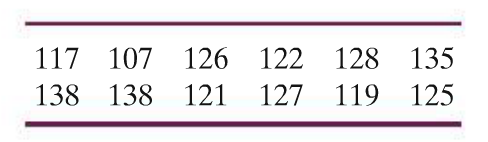
\includegraphics{BoxplotData}
%\end{center}
%
%\noindent
%Use this data to answer the following questions:
%\begin{enumerate}
%	\item Find the \textbf{minimum}, and \textbf{maximum} of the data
%	\item Find the \textbf{25th}, \textbf{50th} and \textbf{75th} percentiles
%	\item What is another name for the 50th percentile?
%	\item Using your graphing calculator calculate the mean, and standard deviation of this data
%	\item Scroll down in your one variable statistics and record the values seen for $Q_1$, $M$, and $Q_3$.
%	\item Compare these values to the values you found in Problem 2.
%	\item Based on your answer to Problems 2, 5 and 6. What conclusions can you make?
%\end{enumerate}
%
%\noindent
%After students complete the warm-up questions we will create a boxplot with the given information. Also define quartiles.\\
%
%\noindent
%Now that we have created a box plot answer the following questions:
%\begin{enumerate}
%	\item How many values are less than $Q_1$?
%	\item How many values are between $Q_1$ and $M$?
%	\item How many values are between $M$ and $Q_3$?
%	\item How many values are greater than $Q_3$?
%	\item Based on the answers you got above and your knowledge of percentiles what sort of generalization can we make about the number of data values that fall less than $Q_1$? between $Q_1$ and $M$? between $M$ and $Q_3$? greater than $Q_3$?
%\end{enumerate}
%
%\noindent
%We will discuss these questions as a class to help us understand the way a box plot and this type measure of center works. As part of this discussion we will also define the Interquartile Range and why it is more useful than the range.\\
%
%\noindent
%Now that we have a box plot we want to see how a box plot relates to a histogram. Use the data from the beginning of the class to answer the following questions:
%\begin{enumerate}
%	\item Create a histogram with a class width of 5 that starts a 105.
%	\item Describe the shape of the histogram.
%	\item Compare the histogram to the box plot. 
%	\item Make a statement about how you can tell the shape of a distribution from a box plot.
%\end{enumerate}
%  
%
%\subsection*{Comparing Boxplots}
%Use these two data sets to answer the following questions:
%
%\[ \text{Data Set 1:} 1, 3, 5, 7, 9, 11, 13, 15, 17\]
%\[ \text{Data Set 2:} 1, 3, 5, 7, 9, 16, 18, 20, 22\]
%
%\begin{enumerate}
%	\item Compare the two data sets: How are they similar? How are they different?
%	\item Draw boxplots for each of these sets of data.
%	\item Compare the min, $Q_1$, M, $Q_3$ and max. How are they similar? How are they different?
%\end{enumerate}
%
%\subsection*{Matching Histograms to Boxplots}
%Match the following histograms to the respective box plots. as an ending activity:
%
%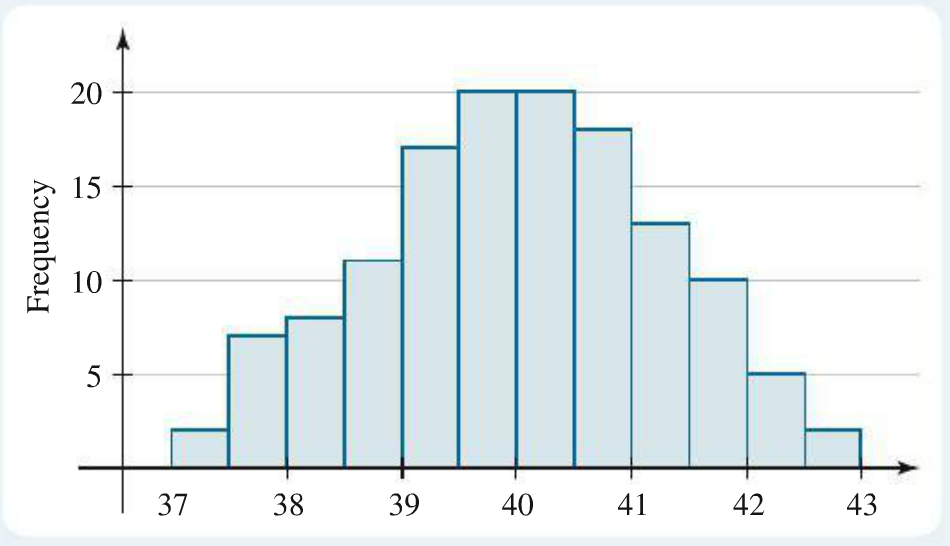
\includegraphics[scale=0.5]{Figure97}
%
%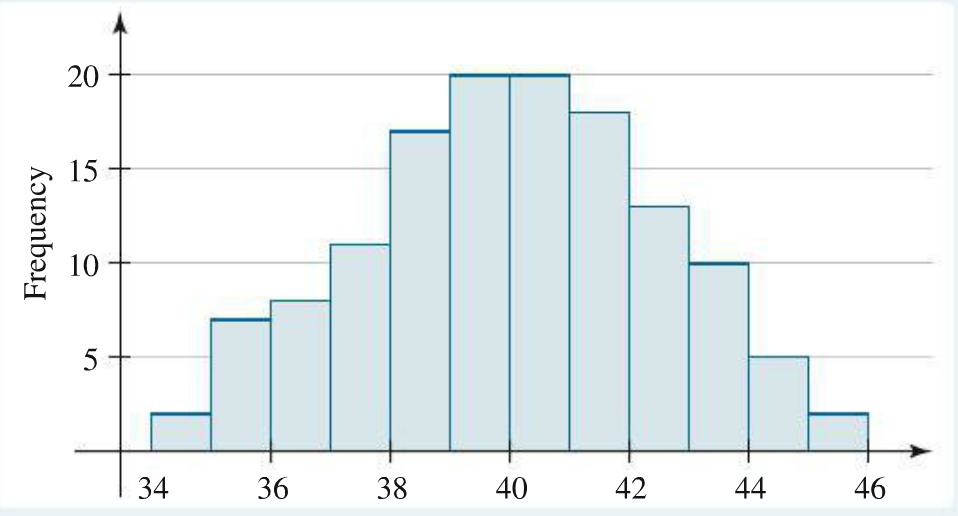
\includegraphics[scale=0.5]{Figure98}
%
%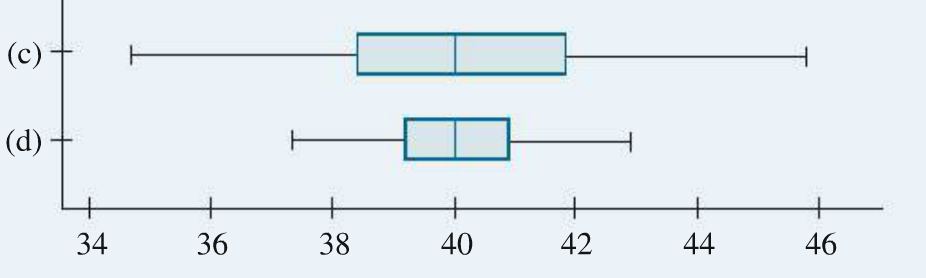
\includegraphics[scale=0.5]{Boxplots}
%
%\newpage
%\noindent
%\section*{Announcements}
%\textbf{Tonight}
%\begin{itemize}
%	\item MyMathLab Section 4.2 due at 11:30pm
%\end{itemize}
%
%\textbf{Thursday, February 8}
%\begin{itemize}
%	\item Quiz 2 in class \textbf{bring your laptop}
%	\item MyMathLab Section 4.3 due at 11:30pm
%\end{itemize}
%
%\textbf{Sunday, February 11}
%\begin{itemize}
%	\item MyMathLab Review 1 due at 11:30pm
%\end{itemize}
%
%\textbf{Thursday, February 15}
%\begin{itemize}
%	\item \textbf{Exam 1} in class
%		\begin{itemize}
%			\item Pen or Pencil with dark lead
%			\item Calculator
%			\item Catcard
%		\end{itemize}
%\end{itemize}

%%%%%%%%%%%%%%%%%%% Day 9: Section 3.5 and Quiz 2 %%%%%%%%%%%%%%%%%%%

%\section*{Section 3.5 and Quiz 2}
%\subsection*{Warm-up}
%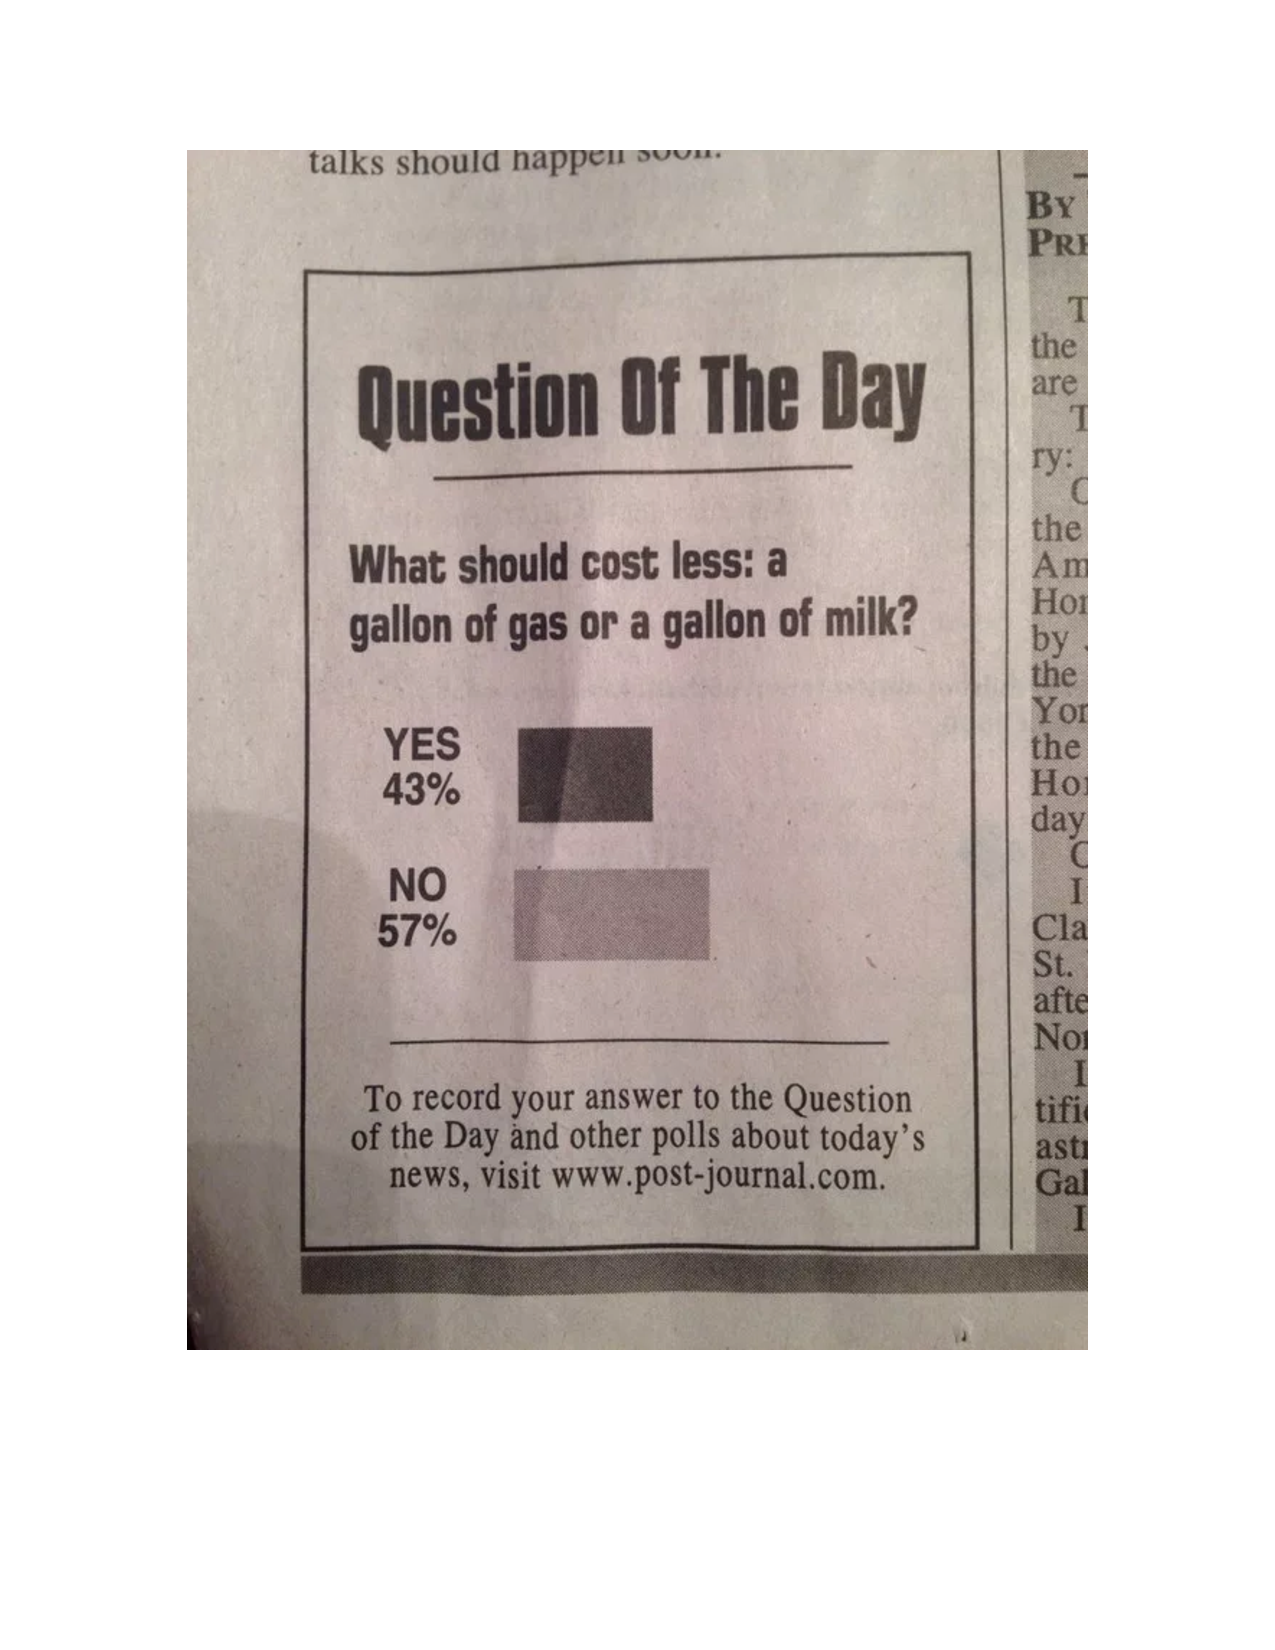
\includegraphics[scale=0.45]{misleadinggraphs.pdf}
%
%\noindent
%Students will discuss each of these and figure out what the creator of the chart wanted you to think and also what  a better way to do the graph.
%
%\subsection*{Class Width of a histogram}
%The following histograms represent the daily high temperatures in San Mateo, California in May of 2014.
%
%\begin{figure}[h!]
%\centering
%\begin{subfigure}{.5\textwidth}
%  \centering
%  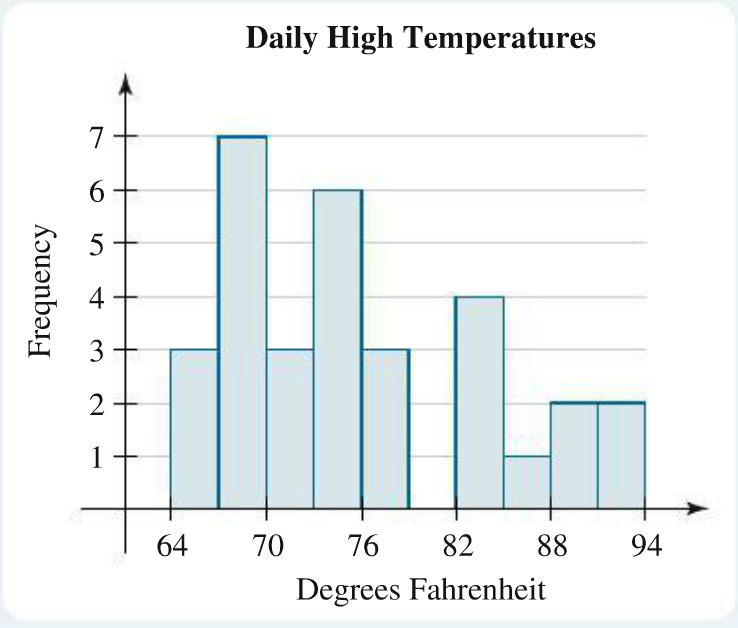
\includegraphics[scale=0.45]{bimodaltemps}
%\end{subfigure}%	
%\begin{subfigure}{.5\textwidth}
%  \centering
%  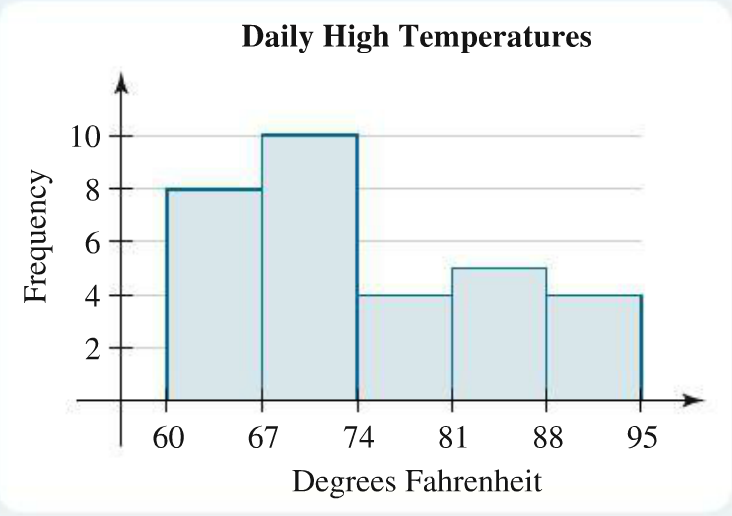
\includegraphics[scale=0.45]{unimodaltemps}
%\end{subfigure}
%\end{figure}
%
%\noindent
%Use these to answer the following questions:
%\begin{enumerate}
%	\item In San Mateo, there tend to be foggy days, and sunny days. Which of these histograms better represents this?
%	\item A person who doesn't like heat is looking into moving to San Mateo, which histogram would be better to show this person?
%	\item What is the difference between the two histograms?
%	\item Would you say that one of these graphs is misleading? How is it misleading?
%\end{enumerate}
%
%\subsection*{Nonuniform Scaling}
%The following chart represents the annual revenue in billions of dollars of Nike.
%
%\begin{center}
%	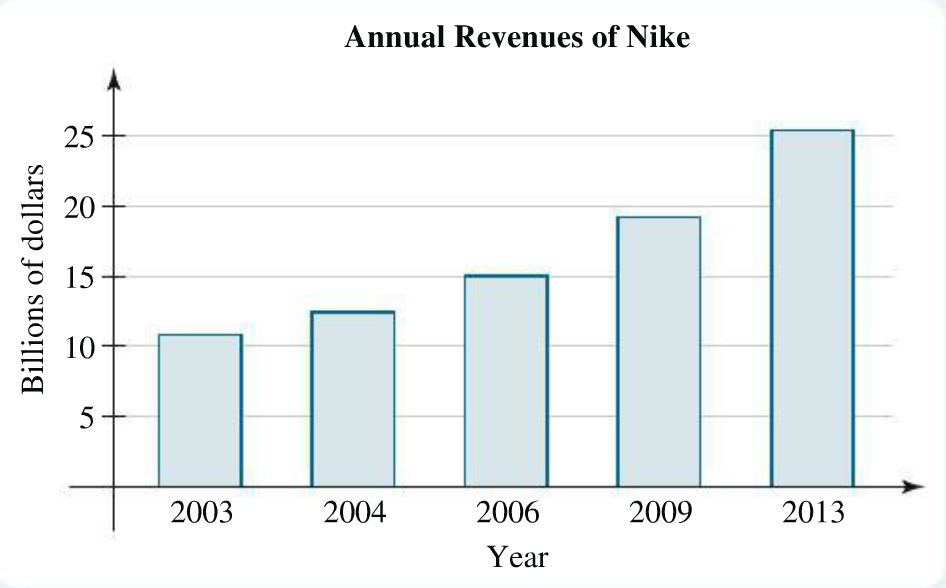
\includegraphics[scale=0.5]{Nikemisleading}
%\end{center} 
%
%\noindent
%Use this graph to answer the following questions.
%\begin{enumerate}
%	\item Based on the graph what would you say about Nike's annual revenue?
%	\item What makes this graph misleading?
%	\item How could you fix it?
%\end{enumerate}
%
%\subsection*{3D Graphs}
%The following bar graph represents wine consumptions of several different countries.
%
%\begin{center}
%	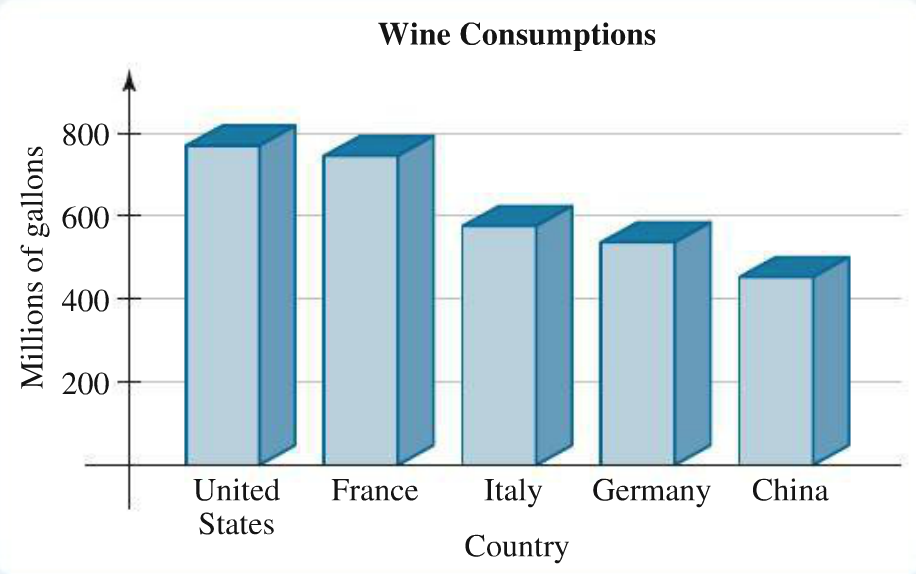
\includegraphics[scale=0.5]{3DMisleading}
%\end{center}
%
%Use this graph to answer the following questions:
%\begin{enumerate}
%	\item Based on the graph which country consumes the most wine?
%	\item What makes this graph misleading?
%	\item How could we fix that problem?
%	\item In addition to the graph being misleading, the data presentation is misleading. What is something about the data presentation that is misleading?
%\end{enumerate}
%
%\subsection*{Time Series Plots}
%The following Time Series Plots represent the United States market shares as a percentage or world manufacturing.
%
%\begin{figure}[h!]
%\centering
%\begin{subfigure}{.5\textwidth}
%  \centering
%  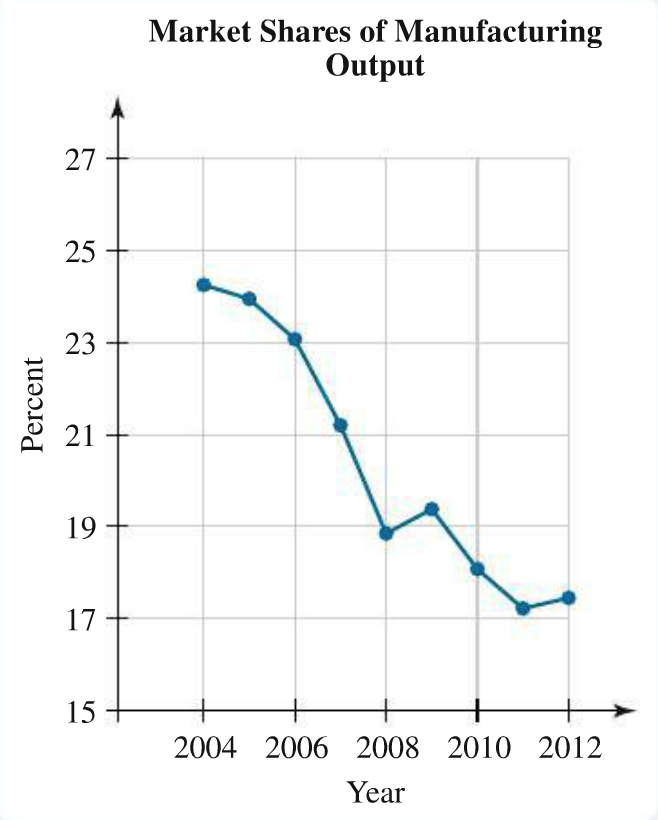
\includegraphics[scale=0.45]{Timeseriesmessedscale}
%\end{subfigure}%	
%\begin{subfigure}{.5\textwidth}
%  \centering
%  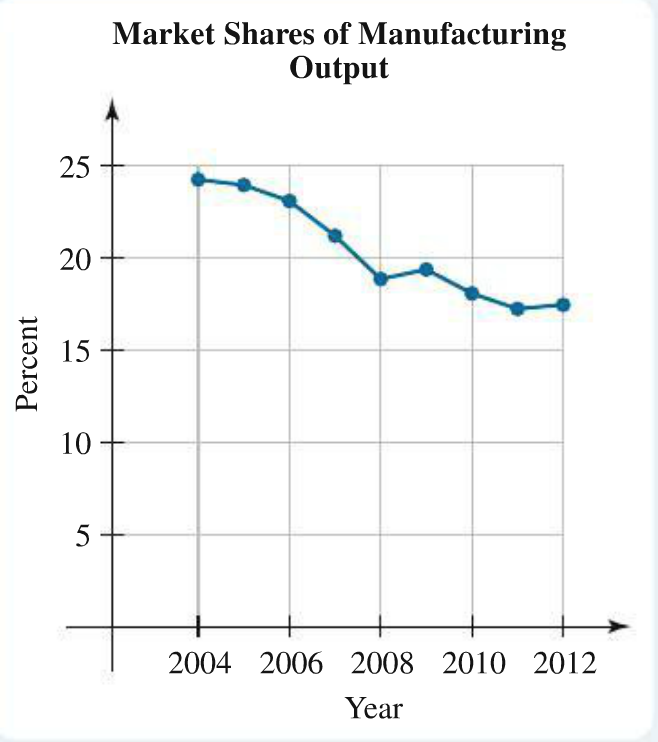
\includegraphics[scale=0.45]{Timeseriesregularscale}
%\end{subfigure}
%\end{figure}
%
%Use these to answer the following questions:
%\begin{enumerate}
%	\item How could the Republican party utilized one of these charts for the 2012 reelection season?
%	\item How could the Democratic party utilized one of these charts for the 2012 reelection season?
%	\item What is the difference between the two time series graphs?
%	\item Would you say that one of these graphs is misleading? How is it misleading?
%\end{enumerate}

%%%%%%%%%%%%%%%%%%% Day 10: Review for Test 1 %%%%%%%%%%%%%%%%%%%

%\section*{Warm-Up}
%Copy the following questions into your notes and then answer the questions.
%\begin{enumerate}
%	\item Is a frequency table used for categorical or numerical data?
%	\item What is an example of a discrete variable? $\ldots$ a numerical variable?
%	\item Do relative frequencies add up to 1 Sometimes? Always? Never?
%	\item Which is bigger? The number of female students at the UA \textbf{\underline{AND}} Female or the number of female students at the UA \textbf{\underline{OR}} Female? How do you know?
%	\item A histogram has 5 classes of class width 3, starting at 14. Write out all the classes.
%	\item Is the 50th percentile the same as the mean? Median? or Neither?
%	\item In a skewed left distribution, which is bigger $\overline{x}$ or $M$?
%	\item In a typical unimodal symmetric distribution, is the more data between $Q_1$ and $Q_3$ or within one standard deviation of the mean?
%\end{enumerate}
%
%\noindent
%After the students discuss a bit, we will have the class answer clicker questions. With luck we will display these for the class and have a discussion based on agreements or disagreements.

%\section*{Review questions}
%\subsection*{Section 3.1}
%A group of 24 students was asked ``If you could have one superpower, what would it be?" The students responses are here.
%\begin{center}
%	\begin{tabular}{llll}
%Mind read   & Fly       & Fly         & Other    \\
%Telekinesis & Fly       & Other       & Teleport \\
%Other       & Other     & Telekinesis & Fly      \\
%Teleport    & Teleport  & Invisible   & Other    \\
%Other       & Invisible & Fly         & Other    \\
%Mind read   & Other     & Fly         & Other   
%\end{tabular}
%\end{center}
%\begin{enumerate}[label=(\alph*)]
%	\item Construct a frequency table.
%	\item Construct a relative frequency table.
%	\item Construct a frequency bar graph.
%	\item Construct a relative frequency bar graph.
%	\item What proportion of students chose flying?
%	\item What proportions of the students did \textbf{NOT} choose invisibility?
%	\item What proportion of the students chose telekinesis \textbf{OR} mind reading?
%\end{enumerate}
%
%\subsection*{Section 3.2}
%Several people were asked their gender and whether or not they worked. The answers as summarized below:
%\begin{center}
%	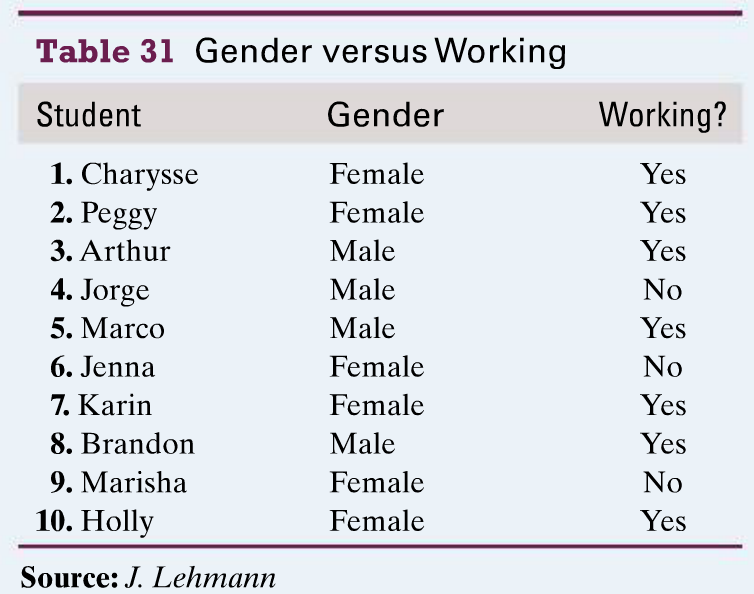
\includegraphics[scale=0.5]{ReviewSec32}
%\end{center}
%Use it to answer the following questions:
%\begin{enumerate}
%	\item Create a two way table that represents gender vs working
%	\item What proportion of students are Female \textbf{\underline{AND}} Work?
%	\item What proportion of students are Female \textbf{\underline{OR}} work?
%	\item Create a multibar graph.
%	\item What proportion of Male students work?
%	\item What proportion of students work?
%	\item What proportion of students are male?
%\end{enumerate}
%
%\subsection*{Section 3.3}
%The following data is the top 50 finishers of the women's New York City Marathon.
%\begin{center}
%	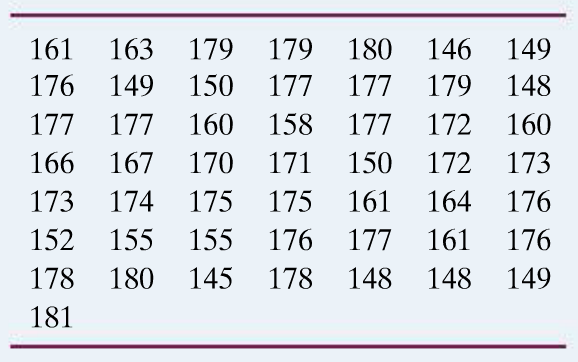
\includegraphics[scale=0.5]{ReviewSec33}
%\end{center}
%Use it to answer the following questions:
%\begin{enumerate}
%	\item Create a stem and leaf plot to represent the data.
%	\item What is the frequency of the observation 148? In context of the problem, what does this mean?
%	\item Which observation has the greatest frequency?
%	\item What type of data is this?
%	\item What is the 87th percentile? What does it represent in this situation?
%	\item How many observations are below 160?
%	\item What percentile is the value 164?
%\end{enumerate}
%
%\subsection*{Section 3.4}
%The following data is the top 24 hits of smartphone prices on Amazon.
%\begin{center}
%	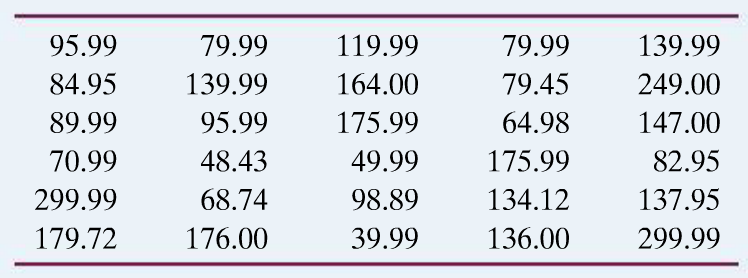
\includegraphics[scale=0.5]{ReviewSec34}
%\end{center} 
%Use it to answer the following questions:
%\begin{enumerate}
%	\item Create a histogram with a class width of 25 and a lower class bound of 25.
%	\item Describe the shape of the distribution.
%	\item Are there any outliers? If so, why is there an outlier?
%	\item What proportion of smartphones have prices between \$95 and \$114?
%	\item Calculate the mean, median, mode, range and standard deviation for this data set.
%\end{enumerate}
%
%\subsection*{Section 4.1}
%\begin{figure}[h!]
%\centering
%\begin{subfigure}{.5\textwidth}
%  \centering
%  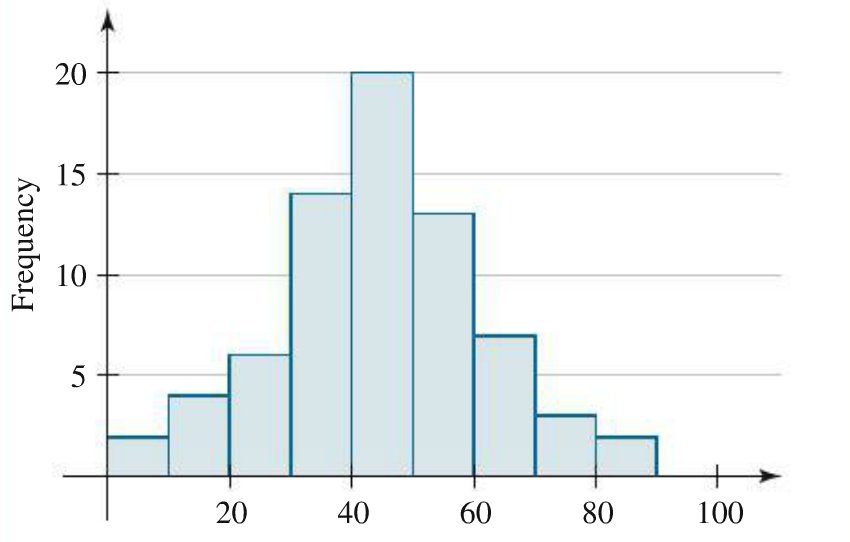
\includegraphics[scale=0.45]{RevSec411}
%  \caption*{(d)}
%\end{subfigure}%	
%\begin{subfigure}{.5\textwidth}
%  \centering
%  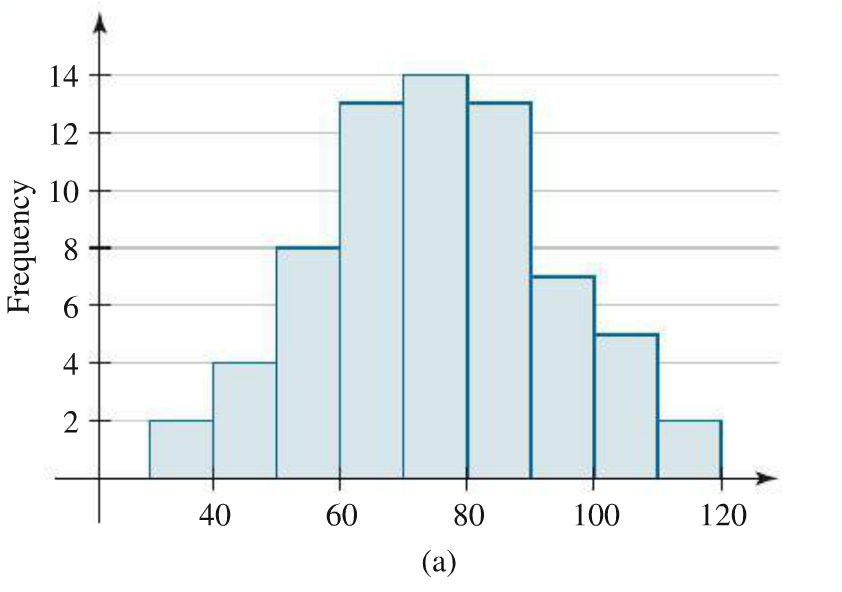
\includegraphics[scale=0.45]{RevSec412}
%\end{subfigure}
%\end{figure}
%
%\begin{figure}[h!]
%\centering
%\begin{subfigure}{.5\textwidth}
%  \centering
%  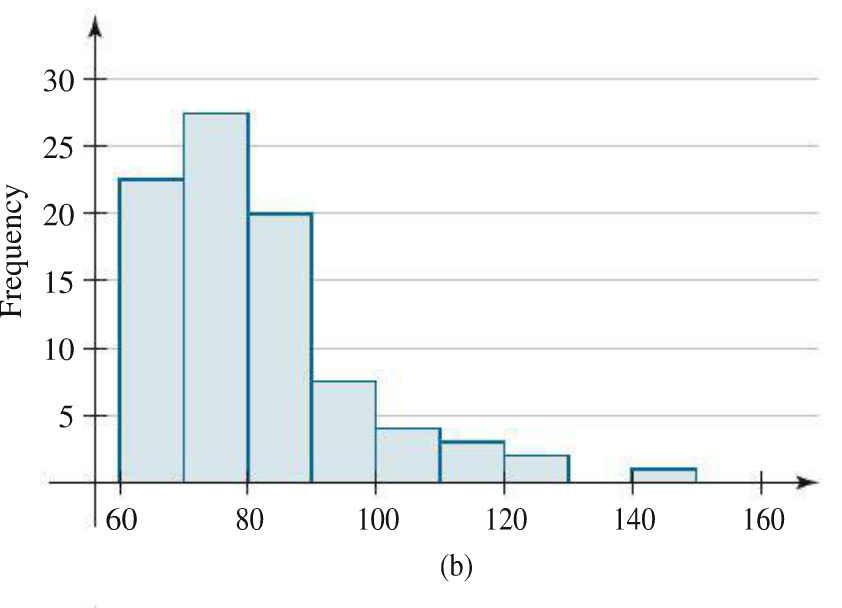
\includegraphics[scale=0.45]{RevSec413}
%\end{subfigure}%	
%\begin{subfigure}{.5\textwidth}
%  \centering
%  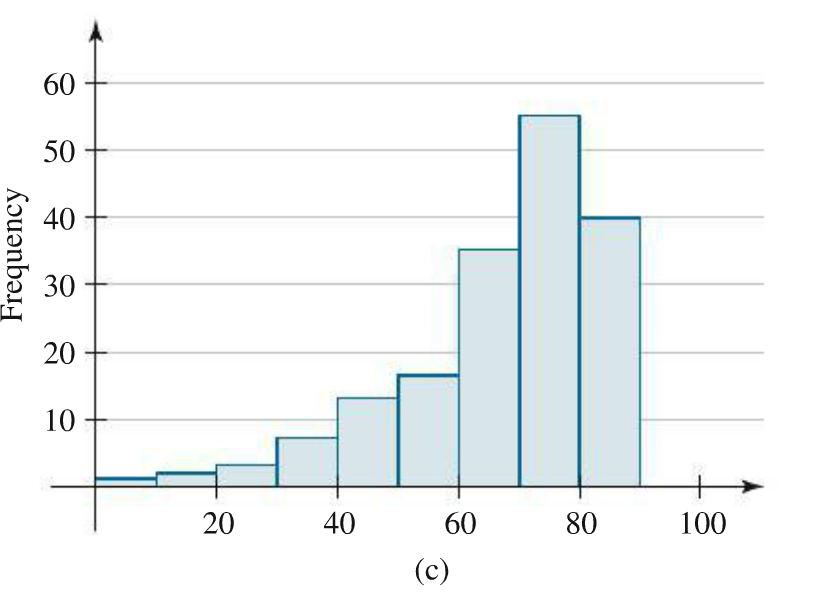
\includegraphics[scale=0.45]{RevSec414}
%\end{subfigure}
%\end{figure}
%
%\noindent
%Use the above to answer these questions.
%\begin{enumerate}
%	\item Describe the shape of each of the histograms
%	\item How is the mean related to the median in each of the histograms?
%	\item Which histograms would we use the mean and standard deviation to describe?
%	\item Which histograms would we use the median and range to describe?
%	\item Estimate the mean and median for each of these histograms.
%\end{enumerate}
%
%\subsection*{Section 4.2}
%\begin{center}
%	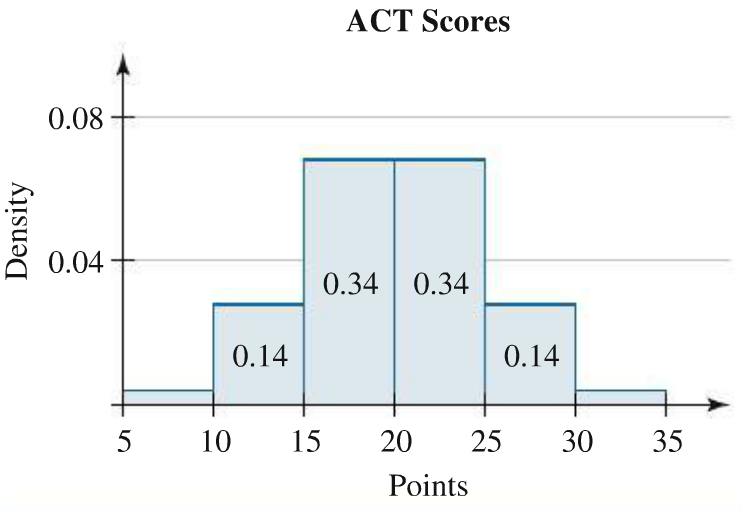
\includegraphics[scale=0.5]{RevSec42}
%\end{center}
%Use this to answer the following questions:
%\begin{enumerate}
%	\item Estimate the proportion of scores that are between 15 and 25 points.
%	\item Estimate the proportion of scores that are between 10 and 30 points.
%	\item Estimate the proportion of scores that are between 5 and 35 points.
%	\item Estimate $s$.
%	\item What rule did you use to estimate $s$? 
%	\item What is another name for the things you calculated in Questions 1, 2 and 3?
%\end{enumerate}
%
%\subsection*{Section 4.2}
%\begin{center}
%	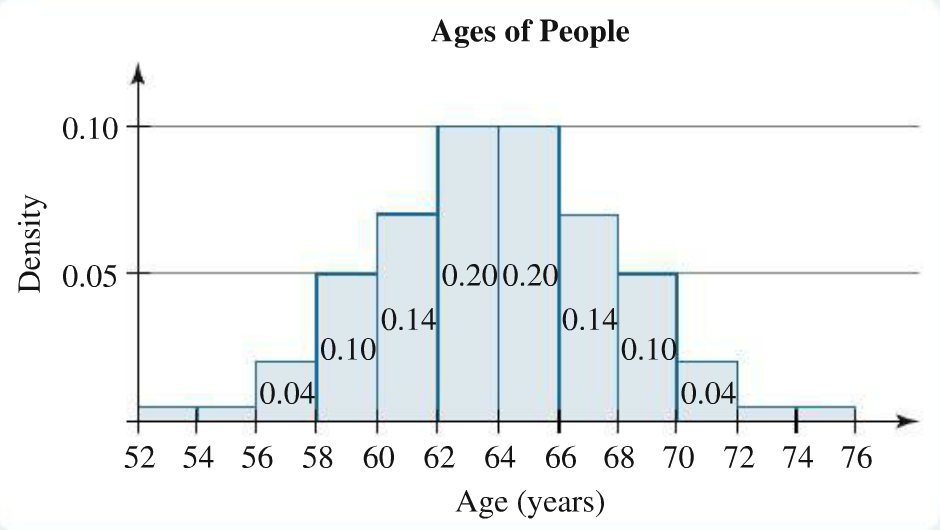
\includegraphics[scale=0.5]{RevSec421}
%\end{center}
%
%\begin{enumerate}
%	\item Estimate $M$
%	\item Estimate $\overline{x}$
%	\item Estimate $s$
%	\item Estimate $R$
%	\item How did you find the answer to Question 3?
%	\item Using your estimate to $s$ and $\overline{x}$ calculate 1, 2 and 3 standard deviations from the mean.
%\end{enumerate}
%
%\subsection*{Section 4.3}
%Use the following boxplot to answer some questions.
%\begin{center}
%	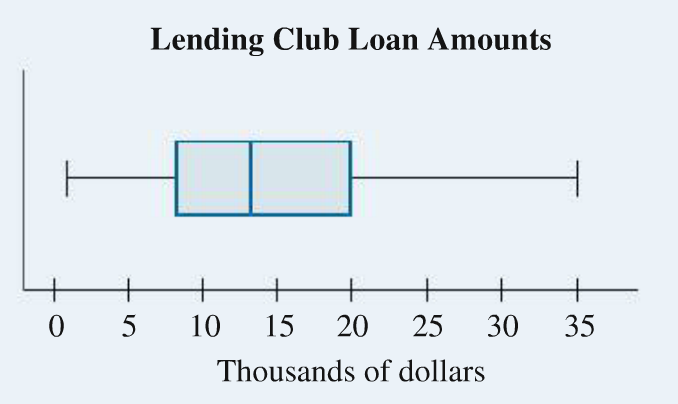
\includegraphics[scale=0.5]{RevSec44}
%\end{center}
%
%\begin{enumerate}
%	\item Describe the shape of the boxplot.
%	\item Estimate the 25th percentile. In context of the problem, what does this mean?
%	\item Estimate the percentile of a \$20 thousand dollar loan. What does this mean in context of the problem.
%	\item What is the largest loan?
%	\item What is the IQR?
%	\item A student says that there are more loans for \$20-\$35 thousand dollars. What would you tell this student?
%	\item How much data is between the loan amounts \$0 and \$8.3 thousand dollars? How do you know?
%\end{enumerate}

%%%%%%%%%%%%%%%%%%% Day 12: Section 5.1 %%%%%%%%%%%%%%%%%%%

%\section*{Section 5.1: Meaning of Probability}
%\subsection*{Warm-Up}
%Students will start by playing rock paper scissors 20 games worth and recording the outcomes. Once they have completed the games they will answer the following questions:
%\begin{enumerate}
%	\item What proportion of times did Player A win? Player B win? Tie?
%	\item List all possible outcomes a round. (i.e. RR for Rock and Rock)
%	\item Is it more likely someone wins or there is a tie? How do you know?
%	\item Is the game``fair"? Why or why not?
%\end{enumerate}
%
%\subsection*{Coin Flip Motivated Intuition Building}
%Now think about a coin flip. Ask students what coin flips are used for and why they use them. Hopefully someone talks about a 50-50 chance of an outcome occurring. From here we will define some terms:
%\begin{itemize}
%	\item Sample space: the group of all possible outcomes
%	\item Event: a group of some of the outcomes (some, none, or all)
%\end{itemize} 
%
%\noindent
%Talk about these definitions in terms of the coin problem and the rock paper scissors activity they started with.\\
%
%\noindent
%Next define probability: Probability of Event E= $\frac{\text{ \# of outcomes in E}}{\text{\# of outcomes in the sample space}}$ Notationally we write $P(E)$.\\
%
%\noindent
%Tie this into proportions/relative frequencies. \textbf{NOTE:} All the language we are using now is just specific to probability but is no different from what we had before. This leads us to know some things about probability all ready. The things we already know:
%\begin{itemize}
%	\item A probability must be between the values of 0 and 1
%	\item The sum of the probabilities of all single events 	is 1
%\end{itemize}
%
%\subsection*{Practicing the Definitions above}
%Think about the Rock Paper Scissors Example we started with at the beginning of class. Use that to answer the following questions:
%\begin{enumerate}
%	\item What is the sample space?
%	\item What does the event A wins contain?
%	\item What is P(A wins)?
%	\item What is P(B wins)?
%	\item What is P(Tie)?
%	\item Is it more likely that someone wins or there is a tie?
%	\item Is the game fair?
%\end{enumerate}
%
%\subsection*{A bit more vocabulary}
%Now think about the coin flip again. 
%\begin{itemize}
%	\item How would you describe the outcomes Head and Tails?\\ \textit{We call the outcomes equally likely when they have the same probability}
%	\item Find P(H and T).\\ \textit{When the probability of the event is 1 we call it a sure event}
%	\item Find P(neither H nor T)\\ \textit{When the probability of the event is 0 we call it impossible}
%\end{itemize}
%
%\subsection*{End Practice Activities}
%
%List/Describe the sample spaces for the following experiments:
%\begin{itemize}
%	\item Drawing a card from a deck of cards
%	\item Rolling a 20 sided dice
%	\item Flipping a coin 3 times
%\end{itemize}
%
%\begin{center}
%	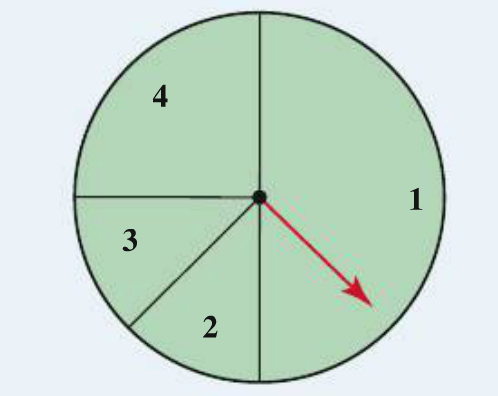
\includegraphics[scale=0.5]{Spinner}
%\end{center}
%Use the spinner to answer the following questions:
%\begin{enumerate}
%	\item Are all outcomes equally likely?
%	\item Give an example of a sure event.
%	\item Given an example of an impossible event.
%	\item Find $P(X=4)$
%	\item Find $P(X\leq 2)$
%	\item Find $P(\text{at least } 2)$
%\end{enumerate}
%
%Consider rolling a six-sided dice once. Answer the following questions:
%\begin{enumerate}
%	\item What is the sample space?
%	\item Are the outcomes equally likely?
%	\item Give an example of a sure event.
%	\item Give an example of an impossible event.
%	\item Find $P(X=2)$
%	\item Find $P(3 \leq X \leq 6)$ 
%	\item Find $P(\text{at most } 4)$
%	\item Find $P(2<X<5)$
%\end{enumerate}

%%%%%%%%%%%%%%%%%%% Day 13: Section 5.2 %%%%%%%%%%%%%%%%%%%

%\section*{Section 5.2: Complement and Addition Rule}
%\subsection*{Warm-Up}
%The students will complete the spinner activity to build intuition into probability specifically the OR rule of probability.\\
%\begin{center} 
%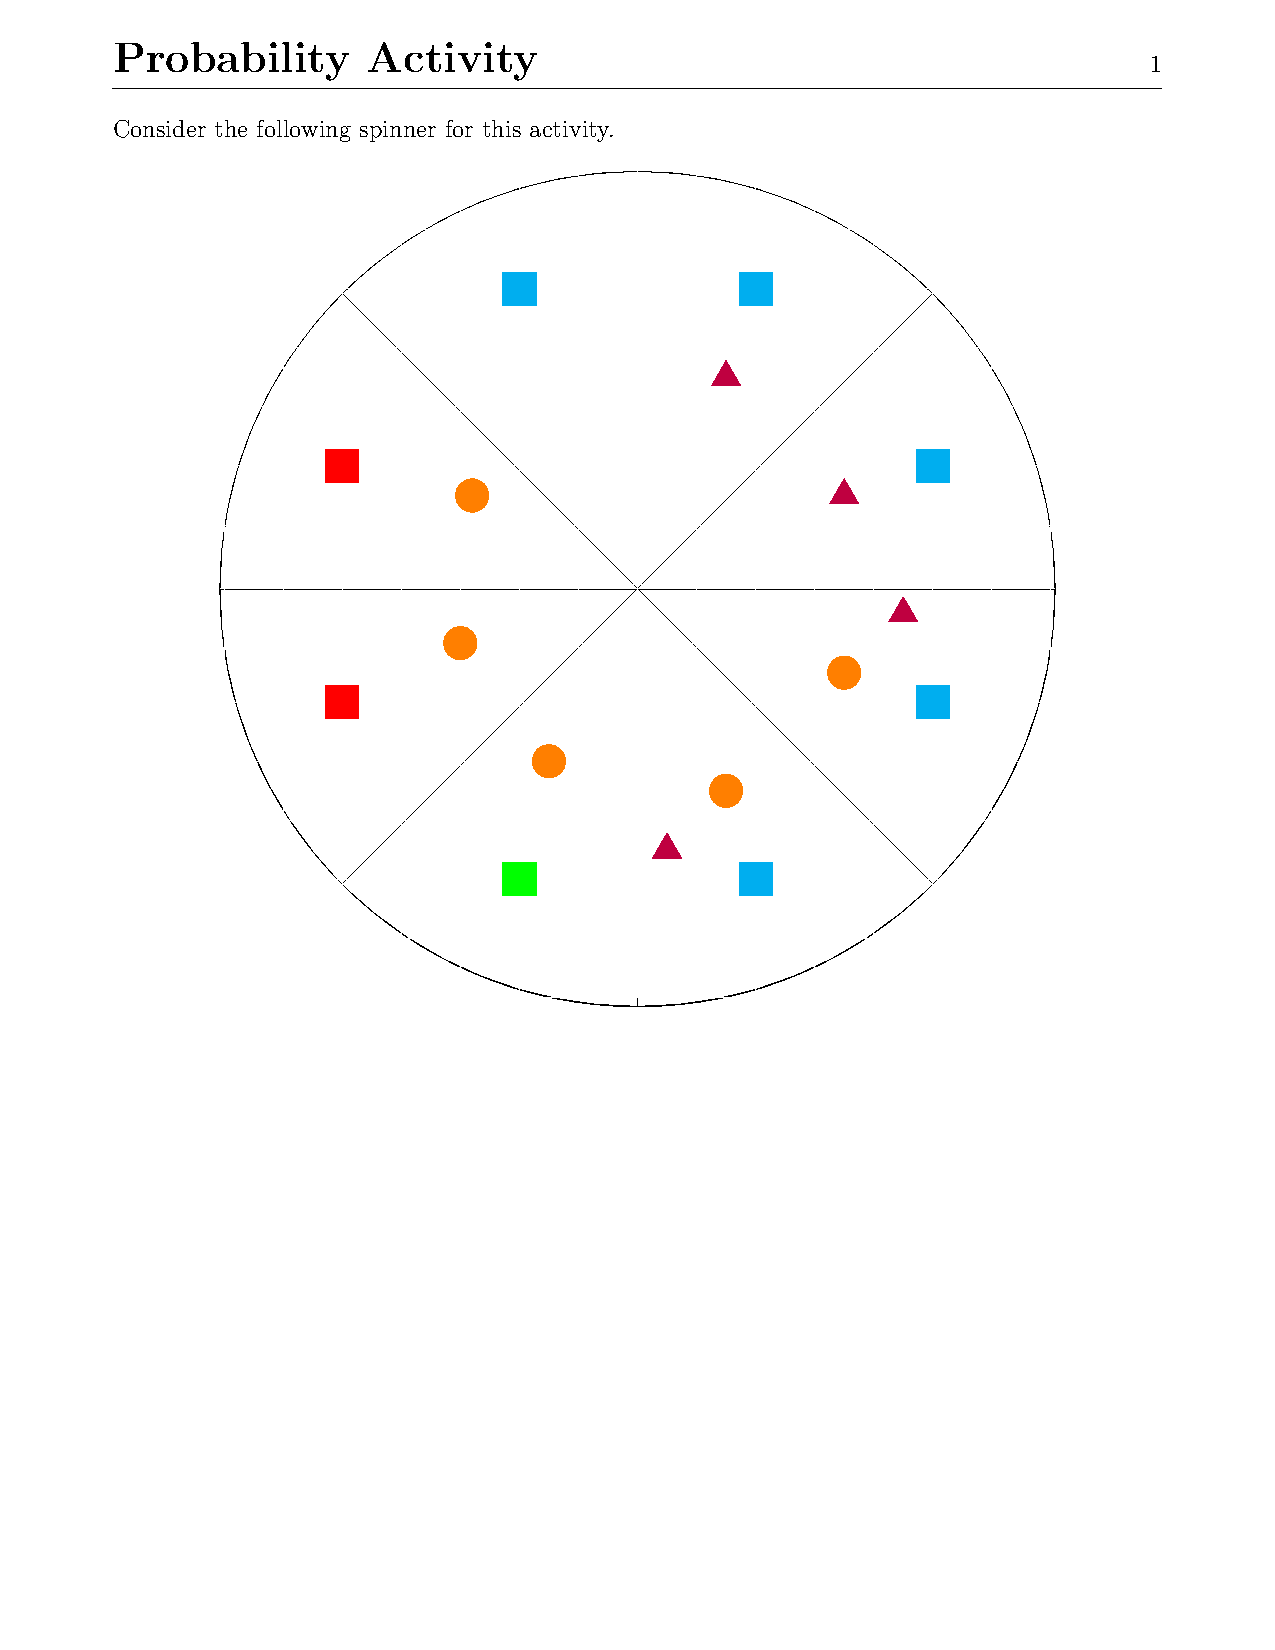
\includegraphics[scale=0.25]{ProbabilityIBLActivity}
%\end{center}
%
%\subsection*{Discussion about Warm-up}
%The warm up is designed to build intuition regarding the formula for OR probability. Once the students have had an adequate time to work on the activity we will regroup to discuss these questions.
%\begin{enumerate}
%	\item We first will discuss questions 1-8 with clicker responses. I will display them on the overhead projector so we get a sense of how the class is doing.
%	\item Next we will discuss as a class the last problems. These are more involved and will require a more in depth discussion. With good luck the students will come up for the formula for OR probability.
%	\item After the discussion of the problems the students completed we will discuss the following definitions:
%		\begin{enumerate}
%			\item Disjoint/Mutually Exclusive Events
%			\item Addition Rule	
%		\end{enumerate}
%\end{enumerate}
%
%\subsection*{Activity for NOT rule}
%Answer the following question regarding rules about probability.
%\begin{enumerate}
%	\item 25.45\% of the students in our class are majoring in Political Science. Use this to answer the following questions:
%	\begin{enumerate} 
%	\item What is the probability that if we were to select a random student from our class that they are a political science major?
%	\item What is the probability that if we were to select a random student from our class that they are \textbf{NOT} a political science major?
%	\end{enumerate}
%	\item 60\% of the students in our class our freshman. What is the probability that if we were to select a random student from the class they are \textbf{NOT} a freshman?
%	\item Based on the previous two questions, what sort of rule can you come up with to calculate the probability of an event \textbf{NOT} happening?
%\end{enumerate}
%
%\subsection*{Discussion about NOT}
%The previous activity is designed to create intuition regarding the formula for NOT probability. Once the students have had adequate time to work on the activity we will regroup to discuss these questions.
%\begin{enumerate}
%	\item The first 3 questions we will use clickers to answer.
%	\item The last question we will discuss as a class.
%\end{enumerate}
%
%\noindent
%At this point we are at the end of the new material for the section. However, over the past two days we have learned a lot of new vocabulary words and ideas so we will continue until about 10 til working with practice problems.
%
%\begin{problem}{}
%Use the following pie chart regarding a survey conducted about social medias influence on purchasing decisions to answer some questions.
%\begin{center}
%	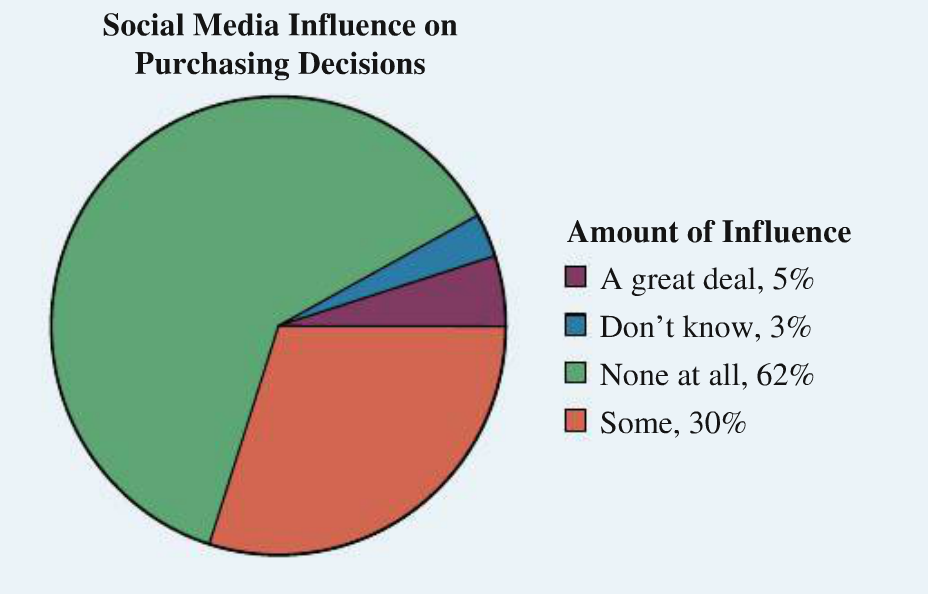
\includegraphics[scale=0.5]{Piechartforprobpractice}
%\end{center}	
%\noindent
%Let $N$ be the event None at all and $S$ be the event some.
%\begin{enumerate}[label=\rm{(\alph*)}]
%	\item Find $P(N)$
%	\item Find $P(S)$
%	\item What is $P( N \textbf{ OR } S)$?
%	\item What is $P( \textbf{NOT } S)?$
%	\item From inspecting the data a student concludes that 62\% of all American adults think that social media has no impact on their purchasing demands. What would you tell this student?
%\end{enumerate}
%\end{problem}
%
%\begin{problem}
%	Use the following chart to answer some questions about probability.
%	\begin{center}
%		\includegraphics[scale=0.5]{Probpractice}
%	\end{center}
%	Let $A$ be the event Agree, $T$ be the event 18 -- 29, $F$ be the event 50 -- 64.
%	\begin{enumerate}[label=\rm{(\alph*)}]
%		\item Find P(A)
%		\item Find P(A \textbf{OR } T)
%		\item Find P(\textbf{NOT } F)
%		\item Find P(A \textbf{AND} T)
%	\end{enumerate}
%\end{problem}
%
%\begin{problem}
%	\item Think of two events that are mutually exclusive.
%	\item Think of two events that are disjoint.
%	\item Think of two events that are not disjoint.	
%\end{problem}
%
%\subsection*{End of class}
%For the remainder of class we will discuss the commonly missed problems on Exam 1. Specifically problems 1 part (b), 3 part (d), problem 7 part (a), problem 5 part (c)

%%%%%%%%%%%%%%%%%%% Day 14: Section 5.4 and Quiz 3 %%%%%%%%%%%%%%%%%%%

%\section*{Section 5.4 Finding Probabilities for a Normal Distribution}
%\subsection*{Motivating Example}
%Several semesters ago, Candace and Zach were taking SBS 200 in the same semester. On their first exam Candace scored a 66.4 out of 83 points and Zach scored a 268.8 out of 336. Candace claims that she did better on the exam than Zach but Zach disagrees. It is our job today to figure out who did better on the exam.\\
%
%\noindent
%As a warm-up, the students will compute the students percentage and discover that they both scored an 80\%. This should be a quick calculation for them.\\ 
%
%\noindent
%Not to be deterred Candace and Zach both talked to their instructors and found that the data for their exams was symmetric and unimodal. Candace found out that her class had a mean of 61 and a standard deviation of 6. Zach found out that his class had a mean of 254 and a standard deviation of 10. Use this information to answer the following questions:
%
%\begin{enumerate}
%	\item Which test was harder? How do you know?
%	\item Did Candace score within one standard deviation of the mean? Did Zach? How do you know?
%	\item Did Candace score within two standard deviations of the mean? Did Zach? How do you know?
%	\item Did Candace score within 3 standard deviations of the mean? Did Zach? How do you know?
%	\item How many standard deviations above the mean did Candace score?\\ How many standard deviations above the mean did Zach score?
%	\item Who did better on the exam?
%\end{enumerate}
%
%\noindent\textit{I would really like students to discover the z-score formula on their own. I don't know if this is possible but maybe it is. I know they will be able to answer questions 1-4 without too much of a problem. Question 5 will be tricky for them. I think that with prompting from us, and the students that have already had a statistics course we will be able to get them there.}
%
%\subsection*{Class discussion about the example}
%The idea we worked with above has a name:
%
%\noindent
%A \textbf{$z$-score} of an observation is the number of standard deviations the observation is from the mean.\\
%
%\noindent
%Some properties of $z$-scores are as follows:
%\begin{itemize}
%	\item $z$-scores are only used with symmetric unimodal data\\ \textit{Note: Ask students to describe/draw with their fingers what symmetric, unimodal distributed data looks like. Draw the smooth curve. State that the curve that we have been drawing over the top of histograms is called the normal distribution and we call the data normally distributed.}
%	\item A $z$-score is found with the following formula \[z=\frac{x-\overline{x}}{s}\]
%	\item An observation that is greater than the mean has a positive z-score
%	\item An observation that is less than the mean has a negative z-score
%\end{itemize}
%
%\subsection*{Practice Calculating $z$-scores}
%Assume that all of the following data sets are normally distributed. Calculate and interpret the $z$-score for the following scenarios: 
%\begin{enumerate}
%	\item Observations: The lengths of songs, in seconds,  played on \textit{Live 105} on April 18, 2014\\ $\overline{x}=232.92$\\ $s=46.93$\\ Coldplay song of 285 seconds
%	\item Observations: Temperature at the top of every hour in February 2014 in Tucson, Arizona\\ $\overline{x}=64.6^{\circ}F$\\ $s=12.2^{\circ}F$\\ The coldest observed temperature of $27^{\circ}F$
%	\item Observations: IQ scores\\ $\overline{x}=100$\\ $s=15$\\ Kim Ung-yong, a Korean child prodigy has an IQ score of 210
%	\item Observations: IQ scores\\ $\overline{x}=100$\\ $s-15$\\ The $z-$score of George Washington is estimated to be 2.167 and the $z-$score of Abraham Lincoln is estimated to be 2.667. What are their corresponding IQ's?
%\end{enumerate}  
%
%\subsection*{Relating Back to Probability}
%So why talk about $z$-scores in the Probability section $\ldots$
%
%\begin{enumerate}
%	\item What does it mean to have a $z$-score of 0?
%	\item What is the probability that a random observation has a negative $z$-score?
%	\item What is the probability that a random observation has a positive $z$-score?
%	\item What is $P(-1 <z<1)$?
%	\item What is $P(-2<z<2)$?
%	\item What is $P(-3<z<3)$?
%\end{enumerate}
%
%\subsection*{Quiz 3}
%Last 30 minutes

%%%%%%%%%%%%%%%%%%% Day 14: Section 5.5 %%%%%%%%%%%%%%%%%%%
%\section*{Section 5.5}
%Last lecture lesson was cut short by the quiz so we will spend the first part of class finishing that material. The warm-up will be the practice calculating the $z$-scores and then the first discussion problem will be the relating back to probability question from the end of last class. After the relating back to probability have a debrief regarding the relationship between ``area under the normal curve" vs. probability.
%
%\subsection*{Guided Probability Practice}
%\textit{Continuation of the last discussion}\\
%
%\noindent
%What is the probability that a randomly selected observation from a collection of normally distributed data that a $z$-score is less than 1?\\
%
%\noindent
%\textit{This question can't be answered by methods we have used up to this point in time. The students will need to use the $z$-score charts. Have them draw a picture and conclude that they might need an additional tool. Pass $z$-score charts out to the groups and read the chart together.}\\
%
%Answer the following questions with your group regarding $z$-scores:
%\begin{enumerate}
%	\item $P(z<1.22)$
%	\item $P(z>1.22)$
%	\item $P(z<-0.45)$
%	\item $P(-0.45<z<1.22)$
%	\item $P(z<-0.45 \textbf{ OR } z>1.22)$
%\end{enumerate}
%
%\subsection*{Practicing with finding probabilities from word problems}
%\textit{Up to this point in time, the students have only worked on finding $z$-scores from data that had already been standardized for them. This problem is geared towards helping them realize the process of translating to a $z$-score and then using the table}\\
%
%\noindent
%Work with your group to answer the following questions:\\
%
%\noindent
%\begin{enumerate}
%	\item Observations: The lengths of songs, in seconds,  played on \textit{Live 105} on April 18, 2014\\ $\overline{x}=232.92$\\ $s=46.93$\\ What is the probability that you tuned into the radio and listened to a song that is 220 seconds long?
%	\item Observations: Temperature at the top of every hour in February 2014 in Tucson, Arizona\\ $\overline{x}=64.6^{\circ}F$\\ $s=12.2^{\circ}F$\\ What is the probability that you experienced a temperature that was greater than $36^{\circ}$?
%	\item Observations: IQ scores\\ $\overline{x}=100$\\ $s=15$\\ Nicole Kidman has  an IQ of 132 and Shakira has an IQ of 140. What is the probability that if we were to pick a random person they would have an IQ score between 132 and 140?
%\end{enumerate} 
%
%\subsection*{A couple of challenging problems to get the students thinking}
%\begin{enumerate}
%	\item A pizza restaurant claims that its mean deliver time is 30 minutes with a standard deviation of 4. An undercover shopper times the amount of time it takes to get her pizza delivered which takes 40 minutes. Is the 40 minute delivery an unusual event?
%	\item For students that graduated high school in 2017 had a mean combined score of  1060 and a standard deviation of 195. Jacque a freshman this year had a combined score of 1320. Is this an unusual score? What is Jacque's percentile?
%	\item For students that graduated high school in 2017 had a mean combined score of  1509 and a standard deviation of 102. Eloise, graduated in 2010 this year had a combined score of 1680. Is this an unusual score? What is Eloise's percentile?
%	\item Using the two questions above what is the probability that a randomly selected student from last years graduating class had a score between Jacque and Eloise?
%\end{enumerate}
%
%\subsection*{Good problem to work on if there is time}
%\includegraphics[scale=0.5]{Gradeonacurve}



%%%%%%%%%%%%%%%%%%% Day 17: Review for Test 2 %%%%%%%%%%%%%%%%%%%

%\section*{Warm-Up}
%Copy the following questions into your notes and then answer the questions.
%\begin{enumerate}
%	\item The probability of an impossible event is?
%	\item The sum of the probabilities of all the single outcome events in the sample space is equal to?
%	\item If two events are disjoint then they share outcomes sometimes? always? never?
%	\item The total area under the normal curve is?
%	\item The $z$-score of an observation is the number of standard deviations an observation is away from the$\ldots$
%	\item If an observation is larger than the mean then it's $z$-score is $\ldots$
%	\item Two sets of data are normally distributed with the same mean. Data set $A$ has a standard deviation of 2.5. Data set $B$ has a standard deviation of 5. The normal curve that represents data set $A$ will be skinnier and taller? shorter and wider? than data set $B$
%	\item True or False: Changing the mean of a normal curve affects the width and height of a normal curve.
%	\end{enumerate}
%
%\noindent
%After the students discuss a bit, we will have the class answer clicker questions. With luck we will display these for the class and have a discussion based on agreements or disagreements.
%
%\section*{Review questions}
%\subsection*{Section 5.1}
%Let $X$ be the outcome of rolling a 9-sided die once. Find the given probability in fraction form:
%\begin{enumerate}
%	\item What is the sample space?
%	\item $P(X=6)$
%	\item $P(X>3)$
%	\item $P(X<5)$
%	\item $P(X\leq 7)$
%	\item $P(X \geq 4)$
%	\item $P(3 \leq X \leq 7)$
%	\item $P(4 \leq X \leq 9)$
%	\item P(odd \textbf{OR} at most 2)
%	\item P(even \textbf{AND} at most 7)
%\end{enumerate}
%
%\subsection*{Section 5.5}
%A total of 940 healthy, pregnant women between 20 and 34 years of age participated in a study. The distribution of their pregnancies was symmetric and unimodal with a mean of 278 days and standard deviation of 8 days. Find the probabilities that a women from the study had a pregnancy that lasted:
%\begin{enumerate}
%	\item less than 260 days
%	\item more than 289 days
%	\item between 265 and 297 days
%	\item A baby that is born in the 8.7th percentile is considered premature and at risk of serious health complications. After what day is a baby no longer considered premature?
%\end{enumerate}
%
%
%\subsection*{Section 5.1/5.2}
%Use the spinner to find the following probabilities:
%\begin{center}
%	\includegraphics{Spinner}
%\end{center}
%\begin{enumerate}
%	\item P(1)
%	\item P(2)
%	\item P(3)
%	\item P(4)
%	\item Are all outcomes equally likely?
%	\item P(odd number)
%	\item P(even number)
%	\item P(not 2)
%	\item P(at least 2)
%	\item P(at most 4)
%	\item What type of event would you call at most 4?
%\end{enumerate}
%
%\subsection*{Section 5.2}
%The following table represents the results of a survey which asked people if they thought their values were threatened by Hollywood and the entertainment industry.
%\begin{center}
%	\begin{tabular}{lllll|l}
%         & 18-29 & 30-49  & 50-69  & over 69 & Total  \\
%Agree    & 1400  & 4847   & 4823   & 3910    & 14,980 \\
%Disagree & 2842  & 6976   & 5661   & 4236    & 19,715 \\ \hline
%Total    & 4242  & 11,823 & 10,484 & 8146    & 34,695
%\end{tabular}
%\end{center}
%Use the table to answer the following questions:
%\begin{enumerate}
%	\item Find the probability that a randomly selected person agreed with the statement.
%	\item Find the probability that a randomly selected person was between 30 and 49 years of age.
%	\item Find the probability that a randomly selected person was 18-29 years of age \textbf{OR} over 69.
%	\item Find the probability that a randomly selected person was 50-59 years of age \textbf{AND} disagreed with the statement?
%	\item Find the probability that a randomly selected person was 50-59 years of age \textbf{OR} disagreed with the statement? 
%\end{enumerate}
%
%\subsection*{Section 5.4}
%\begin{problem}{1}
%	Battery lifetime is normally distributed with an average lifetime of 500 hours with a standard deviation of 61 hours. A package of batteries that Justin recently bought to use with his earphones appears to have batteries that last for 30 days. Find the z-score of the package of batteries that Justin bought. \textbf{Make sure your units match.}
%\end{problem}
%
%
%\begin{problem}{2}
%	A shoe manufacturer is gathering information regarding men's shoe sizes. The company found that men's shoe sizes are normally distributed with a mean size of 11 and a standard deviation of 1.5. Dylan recently went to buy shoes before starting summer classes. He bought shoes of size 9. Find the z-score for Dylan's shoe size.
%\end{problem}
%
%
%\begin{problem}{3}
%	 Windows Surface tablets have a mean battery life of 50 hours and a standard deviation of 12 hours. Stephanie wanted to see if her tablet fell within a ``normal range" and measure how many hours she went before having to recharge her tablet. She found that her tablet would work for 35 hours before needing to be recharged. Find the z-score for Stephanie's tablet.
%\end{problem}
%
%
%\begin{problem}{4}
%	Recently Nathaniel broke a string on his cello and had to replace it. When he went into the store to buy a new string the clerk told him that the lifetime of the string was normally distributed with a mean lifetime of 5 years and a standard deviation of 1.2 years. Nathaniel's last string lasted for 7.5 years. Find the z-score for that strings life.
%\end{problem}
%
%\subsection*{Section5.4}
%
%\begin{problem}{5}
%	Kayla is a triathlon athlete. In the last triathlon Kayla participated in she finished the swimming portion in 53.2 minutes. After talking to the officials she found that the data was normally distributed with an average swimming time of 44 minutes and a standard deviation of 6 minutes. Find the z-score of Kayla's swimming time. 
%\end{problem}
%
%
%\begin{problem}{6}
%	In her nursing class Alyssia learned that the number of hours that Advil is effective for is normally distributed with a mean time of effectiveness of 4.7 hours and a standard deviation of 45 minutes. Alyssia knows from her own experience that when she takes Advil she won't have to take it again until 6 hours later. Find the z-score of the effectiveness of Advil for Alyssia. 
%\end{problem}
%
%
%\begin{problem}{7}
%	In Hawaii, Maggie was part of a gym. It turns out the number of minutes people spend at the gym are normally distributed with an average time of 90 minutes and a standard deviation of 20 minutes. Maggie typically stays for 75 minutes. Find the z-score of how long Maggie stays at the gym.	
%\end{problem}
%
%\begin{problem}
%	A certain cooking sauce is sold in jars marked that they contain 500 grams of sauce. The jars are filled by a machine. The actual weight of the sauce is normally distributed with a mean of 505 grams of sauce with a standard deviation of 2.4 grams. What is the z-score of a jar that weighs 500 grams?	
%\end{problem}
%
%\subsection*{Section 5.5}
%\begin{problem}
%	The 2014 draft picks for NBA basketball teams have heights that are approximately normally distributed with mean 79.1 inches and standard deviation 3.0 inches. The $z$-score for the tallest 2014 draft pick, Walter Tavares, is 2.63. What is Tavares's height? Round to the ones place.
%\end{problem}
%
%\begin{problem}
%	The hourly temperatures at Eppley Airfield Airport in Omaha, Nebraska, in May 2014 are approximately normally distributed with a mean of 64.4$^\circ$F and standard deviation 12.2$^\circ$F. The $z$-score of the highest temperature is 2.59. What is the highest temperature?	
%\end{problem}
%
%\begin{problem}
%	The lengths of songs played on Friday, April 18, 2014 on Live 105. The lengths of the songs are approximately normally distributed with mean 232.93 seconds and standard deviation 49.63 seconds. The shortest song played was ``Fell in Love with a Girl" by the White Stripes. The song's length has a $z$-score of -2.48. What is the length of the song?
%\end{problem}
%
%\begin{problem}
%	The age distribution of inmates on death row in Alabama is approximately normal with mean 43.0 years and standard deviation 9.7 years. The $z$-score of the youngest inmate is -2.16. What is his age?
%\end{problem}
%
%
%
%\subsection*{Section 5.5}
%A professor gives a test to a trigonometry class. The scores are approximately normally distributed with mean 78 points and standard deviation 7 points.
%\begin{enumerate}
%	\item The professor usually uses 90 points as the cutoff for an A. If the professor uses this cutoff, what percentage of the students would get As?
%	\item The professor usually uses 75 to 89 points as the cutoff for a B. If the professor uses this cutoff, what percentage of the students would get Bs?
%	\item The professor usually uses 0 to 45 for an F. If the professor uses this cutoff, what percentage of the students would get Fs?
%	\item If the professor decides to give As to approximately 8\% of the students but not less than 8\%, what should the cutoff score for an A be?
%	\item The professor also decides to gives Fs to approximately 6\% of the students but not less than 6\%, what should the cutoff score for an F be?
%	\item The professor decides to give Bs to students who score above the 65th to 92nd percentiles. What should the cutoff for B be?
%\end{enumerate}
%
%\subsection*{Section 5.5}
%Scores on the Wechsler IQ test are normally distributed with mean 100 points and standard deviation 15 points.
%\begin{enumerate}
%	\item A student's IQ is at the 95th percentile. Find the student's IQ score.
%	\item Mensa is a high-IQ society. Membership is open to people who have attained a score within the upper 2 percent of the general population on an approved intelligence test. What is the cutoff score on the Wechsler IQ test in order to qualify for Mensa?
%	\item A person scores 130 points on the Wechsler IQ test. Is this an unusual score? Why or why not?
%	\item Alexis Martin, who just turned 3 years old, has an IQ of 160 points. What is her $z$-score? Does she have an unusual IQ?
%	\item A student's IQ is at the 42nd percentile. Find the student's IQ score.
%	\item A student's IQ is at the 54th percentile. Find the student's IQ score.
%	\item A student's IQ is at the 12th percentile. Find the student's IQ score.
%\end{enumerate}

%%%%%%%%%%%%%%%%%%%% Day 19: Section 6.1 %%%%%%%%%%%%%%%%%%%%
%\section*{Section 6.1}
%\subsection*{Warm-Up Question}
%\includegraphics{HousingPricesTucson}
%On their whiteboards at the tables, the students will draw two sets of coordinate axes, with a horizontal axis that starts at 0 and ends at 4000 with tick marks every 500 and a vertical axis that starts at 0 and ends at 900 with tick marks every 100. The students will then plot the points that are given in the data. One of them is made up and the other is actual data from Zillow for houses currently on the market. After they have plotted the points, they  will answer the following questions.
%\begin{enumerate}
%	\item One of the data sets is real, and the other is made up. Based on your plots which one do you think is real? Why?
%	\item Do you think a 2,500 square foot home in Tucson is on sale for \$400,000 currently? If not, what would be a reasonable price for such a house?
%	\item A relator listed a 3,000 square foot home for \$100,000 recently. Give three possible reasons that might explain this data point.
%\end{enumerate}
%
%\subsection*{Discussion}
%Up to this point in time in the class, we have been working with one variable, either categorical or numeric. For the remainder of the semester we are going to be working with and comparing two numeric variables (like we just did).\\
%
%\noindent
%At this point in time I want the students to work together for a couple of minutes to brainstorm things they know about graphs and scatterplots. I will display three scatterplots one with positive association, one with negative association, and one with no association. In this activity we will try to get the students to come up with the following.
%\begin{itemize}
%	\item Horizontal axis: x-axis, independent variable, first coordinate in an ordered pair, explanatory variable
%	\item Vertical axis: y-axis, dependent variable, second coordinate in an ordered pair, response variable
%	\item Positive association: Response variable increases as explanatory variable increases
%	\item Negative association: Response variable decreases as explanatory variable increases
%	\item No association: Association is neither positive nor negative
%\end{itemize}
%
%\subsection*{Practice}
%For each situation:
%\begin{enumerate}[label=\alph*)
%	\item 
%\end{enumerate}

%%%%%%%%%%%%%%%%%%%% Day 21: Section 6.2 %%%%%%%%%%%%%%%%%%%%

%\section*{Section 6.3}
%\subsection*{Warm-up Question}
%The following table represents the overdraft fees collected by banks in certain years since 2000. 
%\begin{center}
%\begin{tabular}{c|c}
%Year & \begin{tabular}[c]{@{}l@{}}Amount of Overdraft Fees\\ (billions of dollars)\end{tabular} \\
%2001 & 22.2                                                                                     \\ \hline
%2003 & 27.1                                                                                     \\ \hline
%2005 & 29.7                                                                                     \\ \hline
%2007 & 34.1                                                                                     \\ \hline
%2009 & 37.1                                                                                    
%\end{tabular}
%\end{center}
%Let $A$ be the total amount (in billions of dollars) of overdraft fees collected in the year that is $t$ years since 2000. Using the whiteboards at your table answer the following questions.
%\begin{enumerate}
%	\item Construct a scatterplot (if you use your calculator make sure to draw a sketch of it)
%	\item Draw a (straight) line that comes close to all of the data points in your scatterplot.
%	\item Use your line to estimate the total amount of fees collected in 2008.
%	\item Use your line to estimate when the total amount of fees collected was \$32 billion.
%	\item Find the point where the line intersects the $A$-axis. What does it mean in this situation?
%	\item Use your line to estimate the total amount of fees collected in 2011. Compare your result with \$31.6 billion, which is the actual amount. \textit{new regulations people must opt in to overdraft fees instead opting for decline of charge instead}
%\end{enumerate}
%
%\noindent
%\textit{After the students we will discuss the answers to 3-6 as a class. For 3,4,5 and the first part of 6 we will use the clickers to get an idea of the numbers that the students find. This will then lead into a discussion about models and linear models}
%
%\subsection*{Vocabulary Discussion for throughout the class}
%\begin{itemize}
%	\item Model: A mathematical description of an authentic situation.
%	\item Linear Model: A nonvertical line that describes the association between two quantities in an authentic situation.
%	\item Interpolation: Making an estimation for a data value that falls within the range of $x$-values already provided.
%	\item Extrapolation: Making an estimation for a data value that falls outside the range of $x$-values already provided.
%	\item Model Breakdown: When a model doesn't make sense or an estimate that is not a good approximation
%	\item $x$-intercept: point on the line where the line and the $x$-axis intersect
%	\item $y$-intercept: point on the line where the line and the $y$-axis intersect
%	\item intercept: point on the line where the line and an axis intersect
%	\item Error: the amount in which an estimate differs from the actual value
%\end{itemize}
%
%\subsection*{Example 2}
%The percentages of cell phone users who send or receive text messages multiple times per day are shown for various ages.\\
%
%\begin{center}
%	\begin{tabular}{c|c}
%Age ($a$)  & Percent ($p$) \\ \hline
%21   & 76      \\ \hline
%29.5 & 63      \\ \hline
%39.5 & 42      \\ \hline
%49.5 & 37      \\ \hline
%59.5 & 17     
%\end{tabular}
%\end{center}
%
%\begin{enumerate}
%	\item Determine the explanatory variable and the response variable.
%	\item Draw a scatterplot that represents the data. 
%	\item Describe the shape, association and direction of the association.
%	\item Draw a linear model that fits the data.
%	\item Predict the percentage of 35-year-old cell phone users who send or receive text messages multiple times per day. 
%	\item Find where the graph crosses through the $p$-axis. In context of the problem, what does this mean?
%	\item Find where the graph crosses through the $a$-axis. In context of the problem what does this mean?
%\end{enumerate}
%
%\noindent
%\textit{At this point in time we will define: intercepts (x, y, and just intercept), interpolation, extrapolation and model breakdown}
%
%\subsection*{Example 3}
%The following represents the number of collisions at highway-railroad crossings per year since 1990.
%\begin{center}
%	\begin{tabular}{ll}
%Year & Number of Collisions \\
%1992 & 4.9                  \\
%1995 & 4.6                  \\
%2000 & 3.5                  \\
%2005 & 3.1                  \\
%2010 & 2.1                  \\
%2014 & 2.3                 
%\end{tabular}
%\end{center} 
%
%\begin{enumerate}
%	\item Determine which variable is the explanatory variable, and which is the response variable.
%	\item Draw a scatterplot that represents the situation.
%	\item Describe the four characteristics of the association.
%	\item Draw a linear model on your scatter plot.
%	\item Use your model to predict the number of collisions in 2012. Did you perform interpolation or extrapolation?
%	\item Use your model to predict the number of collisions will be 1.0 thousand. 
%	\item Do you have faith in your result? Why or why not?
%	\item Find the $t$-intercept. What does it mean in this situation?
%	\item Do you have faith in your result? Why or why not?
%\end{enumerate}
%
%\noindent
%\textit{After the students have practiced this example, we will go back to the examples from Tuesday's class and think about whether or not a linear model fits the data and if it does, do the intercepts make sense.}

%%%%%%%%%%%%%%%%%%%% Day 22: Section 7.1 %%%%%%%%%%%%%%%%%%%%

%\section*{Section 7.1 Graphing Equations of Lines and Linear Models}
%\subsection*{Warm-Up Question}
%Paul and Judy did some baking this past weekend. At 1 pm Paul realized he forgot to preheat the oven and immediately turned it on. His oven was $75^{\circ}$F and the temperature began to rise $50^{\circ}$F per minute. Judy on the other hand preheated her oven so that at 1pm her oven was $375^{\circ}$F and stayed at this temperature. 
%\begin{enumerate}
%	\item Make a table that represents Paul and Judy's oven temperature for every minute between 1pm and 1:10pm.
%	\item Make a scatterplot for Paul's oven temperature from 1pm to 1:10pm.
%	\item On the same set of axes make a scatterplot for Judy's oven temperature.
%	\item Draw a linear model for Paul's oven temperature.
%	\item How would you describe the association of Paul's oven temperature?
%	\item Using you linear model, estimate when Paul's oven was the same temperature as Judy's oven.
%\end{enumerate}
%
%\noindent
%\textit{This activity is to get students to start thinking about lines and reinforce concepts from last class, since both are exactly linear associations. We will discuss with the students what they did and how they found it. After the discussion we will give the students 1 minute as a group to discuss with their group the general form of a line and what the different pieces mean. This is meant to see where students are with lines. After their discussion we will have a clicker activity to poll the students to see what they come up with. This will inform the rest of the week's instruction.}
%
%\subsection*{Some Notes}
%\textit{At this point, the students have thought about lines a little bit so we can now define the basics of lines that we are covering today}
%
%\noindent
%\begin{itemize}
%	\item Any non-vertical line has the \textbf{equation} $y=mx+b$ where $m$ is the \textbf{slope} and $b$ is the \textbf{y-intercept} of the line.
%	\item A ordered pair $(P,Q)$ is a \textbf{solution} to the equation $y=mx+b$ if the equation is true when $P$ is substituted for $x$ and $Q$ is substituted for $y$. If $(P,Q)$ is a solution to the equation, we say $(P,Q)$ satisfies the equation.
%	\item The \textbf{graph} of $y=mx+b$ is the set of points that correspond to solutions of the equation.
%\end{itemize}
%
%\noindent
%\textit{The following is a small example to illustrate the above concepts. We will do these quickly as a class to help clarify some of the definitions, specifically the solution definition and review things they should already know and get them thinking about the algebra they have seen in the past.}
%Consider the equation $y=2x+1$. 
%\begin{enumerate}
%	\item Does the point $(1,1)$ satisfy the equation? 
%	\item Does the point $(1,5)$ satisfy the equation?
%	\item We can graph the equation by creating a table of values and then plotting those points.
%\end{enumerate}
%
%\subsection*{Some Practice}
%\textit{The students will practice their line skills at their tables.}
%
%\noindent
%\begin{enumerate}
%	\item Find four solutions to the equation $y=-2x+6$ and find four points that do not satisfy the equation.
%	\item On a coordinate axis draw all 8 points and draw the graph of the equation $y=-2x+6$
%	\item Find the $x$ and $y$ intercepts of the equation and label them on your graph.
%	\item Repeat Parts 1 -- 3 from above for the equations $y=2x-2$.
%\end{enumerate}
%
%\subsection*{Example}
%\textit{This example ties this content back to what we have been doing in class with scatterplots}\\[4mm]
%
%\noindent
%Erin Gilbert recorded the number of calls, $N$, the Ghostbusters received over several evenings when the temperature is, $T$, in degrees celsius. The following is what she recorded:
%
%\begin{center}
%	\begin{tabular}{l|lllllll}
%$T$ & 19 & 27 & 21 & 15 & 23 & 11 & 14 \\ \hline
%$N$ & 29 & 13 & 24 & 33 & 18 & 44 & 36
%\end{tabular}
%\end{center}
%
%\begin{enumerate}
%	\item Decide on the explanatory/response variables and \textit{carefully} plot the data.
%	\item Is the association positive, negative or neither.
%	\item Graph the line $y=-2x+63$ on the same set of axes. Does the line come close to the data points.
%	\item Find the $x$ and $y$ intercepts of the equation. In the context of the problem what do they mean?
%\end{enumerate}
%
%\noindent
%\textit{After the students have worked on this problem and we have discussed it we will talk about the slope of the line and define rate of change. The \textbf{rate of change} of a variable $y$ with respect to a variable $x$ is $\frac{\text{change in } y}{\text{change in } x}$. In the previous example the rate of change of the number of calls per night with respect to the temperature is they receive 2 fewer calls per degree celsius. End the discussion with students talking about the opening activity rate of change. What is the rate of change of Paul's oven? Judy's oven?}

%%%%%%%%%%%%%%%%%%%% Day 23: Section 7.2 %%%%%%%%%%%%%%%%%%%%

%\section*{Section 7.2: Rate of Change}
%\subsection*{Warm-up Problems}
%Alfredo works on campus in Residence Life as a desk assistant. For the past few paychecks the he has been keeping track of the amount of money he has earned. The following table summarizes the results: 
%\begin{center}
%	\begin{tabular}{c|c}
%Number of Hours & Paycheck Amount \\ \hline
%20              & \$200           \\
%12.5            & \$125           \\
%9.25            & \$92.5          \\
%10              & \$100          
%\end{tabular}
%\end{center}
%
%\begin{enumerate}
%	\item Draw a scatterplot that represents this situation.
%	\item Identify the 4 characteristics of association
%	\item Find the rate of change between 4 pairs of data points.
%	\item Compare the rates of change you calculated (how are they similar, how are they different)
%\end{enumerate}
%
%\noindent
%The numbers in thousands of service members in the armed forces diagnosed as overweight for various years is shown below.
%
%\begin{center}
%	\begin{tabular}{c|c}
%Years & Number of Overweight Service Members \\ \hline
%2006  & 56                                   \\
%2007  & 62                                   \\
%2008  & 72                                   \\
%2009  & 29                                   \\
%2010  & 86                                  
%\end{tabular}
%\end{center}
%
%\begin{enumerate}
%	\item Draw a scatterplot that represents this situation.
%	\item Identify the 4 characteristics of association
%	\item Find the rate of change between 4 pairs of data points.
%	\item Compare the rates of change you calculated (how are they similar, how are they different)
%\end{enumerate}
%
%Use the examples from above to answer the following questions:
%\begin{enumerate}
%	\item Compare the two data sets. How are they similar? How are they different?
%	\item Make a generalization about the relationship between $r$-values and the rate of change for a linear model.
%\end{enumerate}
%
%\noindent
%\textit{This example is to further the use of rate of change that we talked about in class on Tuesday at the very end of class. Most students will already know that rate of change is defined to be the change in $y$ divided by the change in $x$. The hope is that once the students are done with this example they will see how rate of change is related to a linear model. The exact linear model with an $r$-value of 1 will have the rate of change be the same for all of the data point pairs, a non-exact linear model with an $r$ value that is not $\pm 1$ will have differences between the rates of change with different pairs of the points. The hope of this is also that students will start to see rate of change as a fancy term for slope.}
%
%\subsection*{Discussion}
%\textit{Once students have completed the warm-up activity and we have discussed together, I will ask them to collaborate with their table mates to come up with things they already know about rate of change (my hope is they have already connected it with slope). Once students have discussed we will discuss the following:}
%\begin{itemize}
%	\item Rate of Change = $\frac{\text{change in }y}{\text{change in }x}$ = $\frac{y_2-y_1}{x_2-x_1}$ = slope
%	\item Note: Rate of change = slope only if $r=1$
%	\item Negative vs. Positive rates of change (how they relate to negative vs positive association)
%	\item Horizontal Lines
%	\item Vertical Lines
%\end{itemize}
%
%\subsection*{Practice Problems}
%\textit{For the remainder of the class until the quiz, the students will work on practicing calculating rate of change in a variety of ways. We will emphasize with each table including units, \textbf{this needs to be stressed as most won't include them} and a practical interpretation. I will put up two problems at a time and give students an appropriate amount of time to work on one of the problems, even if they are an even table and odd if they are at an odd table. At the end of the allotted working time, they will share with a nearby table of the opposite parity what they did and how they got their answer. The problems are very similar in nature so this is a good opportunity to have students teach their peers.}
%
%\begin{problem}
%The volume of water in a swimming pool increases steadily by 2400 gallons in an 8-hour period. Find the rate of change of volume of water.
%\end{problem}
%
%\begin{problem}
%	The temperature decreases steadily by $15^\circ$F over a 3-hour period. Find the rate of change of temperature.	
%\end{problem}
%
%\begin{problem}
%	The number of female-owned firms increased approximately steadily from 5.4 million firms in 1997 to 8.6 million firms in 2013. Find the approximate rate of change of the number of female-owned firms.
%\end{problem}
%
%\begin{problem}
%	The number of U.S. cable TV subscribers decreased approximately steadily from 61.8 million subscribers in 2009 to 54.3 million subscribers in 2014. Find the approximate rate of change of the number of U.S. cable TV subscribers.
%\end{problem}
%
%\begin{problem}
%	The scatterplot and the linear model below describe the association between years and the numbers (in millions) of Americans without health insurance.
%	\begin{center}
%		\includegraphics[scale=0.25]{insurance}
%	\end{center}
%	\begin{itemize}
%		\item Describe the direction of the association. What does it mean in the context of the problem?
%		\item Estimate the rate of change of the number of Americans without health insurance.
%	\end{itemize}
%\end{problem}
%
%\begin{problem}
%	The scatterplot and the linear model below describe the association between years and women's 200 meter run record times in seconds.
%	\begin{center}
%		\includegraphics[scale=0.25]{run}
%	\end{center}
%	\begin{itemize}
%		\item Describe the direction of the association. What does it mean in the context of the problem?
%		\item Estimate the rate of change of the number of Americans without health insurance.
%	\end{itemize}
%\end{problem}
%
%\noindent
%\textit{At this point in time it will likely be time for the quiz. Password hamilton}

%%%%%%%%%%%%%%%%%%%% Day 24: Section 7.2 %%%%%%%%%%%%%%%%%%%%

%\section*{Section 7.3: Using Slope to Graph Equations of Lines and Linear Models}
%\subsection*{Warm-up Problems}
%
%Amazon.com's revenues are show below for several years.
%\begin{center}
%	\begin{tabular}{c|c}
%Year & \begin{tabular}[c]{@{}c@{}}Revenue\\ (billions of dollars)\end{tabular} \\ \hline
%2010 & 34.2                                                                    \\
%2011 & 48.1                                                                    \\
%2012 & 61.1                                                                    \\
%2013 & 74.5                                                                    \\
%2014 & 89.0                                                                   
%\end{tabular}
%\end{center}
%
%\noindent
%Define revenue to be $r$ and $t$ to be years since 2010. Use this data and information to answer the following questions:
%\begin{enumerate}
%	\item Create a scatterplot to represent the data on the whiteboard and on your graphing calculator.
%	\item Describe the 4 characteristics of association for this data.
%	\item Calculate the rate of change between 2010-2011, 2012-2014 and 2010-2014.
%	\item A linear model that represents this data is given by $r=13.6t+34.18$. Use your graphing calculator to graph this line for directions using a TI calculator see A.16-A.18 in the text book for instructions on how to do this. Also sketch the line on your scatterplot you drew on the whiteboard.
%	\item Do you think this linear model is a good model for the situation? Why or why not?
%	\item Compare your answers of rate of change to the rate of change in the model. 
%	\item Use the model to predict the revenue in 2019. Did you perform interpolation or extrapolation? Do you have faith in your estimation?
%\end{enumerate}
%
%\subsection*{A little bit of review}
%\textit{These will be used as clicker questions.}
%
%\begin{enumerate}
%	\item What is the slope-intercept form of a line?
%	\item In $y=mx+b$, $m$ represents?
%	\item In $y=mx+b$, $b$ represents?
%	\item What is a slope of the horizontal line?
%	\item What is the slope of a vertical line?
%	\item To calculate rate of change we use the following formula$\ldots$
%\end{enumerate}
%
%\subsection*{Sketching Lines}
%\textit{The following will be done based on table numbers. The even numbered tables will do the even numbered problem and the odd numbered table will do the odd numbered problem. At the end of an appropriate amount of time, I will have the tables discuss amongst themselves. I will at the end allow them 1 minute each time to copy what they feel is necessary into their notes. We won't be discussing this as a class. This means that we need to be proactive in addressing incorrect answers and asking tables questions as they work on the problems}
%
%\begin{enumerate}
%	\item Graph $y=-x+2$
%	\item Graph $y=\frac{5}{2}x-3$
%	\item Graph the line that has $m=\frac{2}{3}$ and passes through the point $(4,-5)$.
%	\item Graph the line that has $m=\frac{-3}{4}$ and passes through the point $(6,3)$.
%	\item Graph the line that has $m=0$ and passes through the point $(2,3)$.
%	\item Graph the line that has $m$ undefined and passes through the point $(1,4)$.
%	\item Graph the line $x=7$
%	\item Graph the line $y=3$
%	\item Graph a line in which $m$ is positive and $b$ is negative.
%	\item Graph a line in which $n$ is negative and $b$ is positive.
%\end{enumerate}
%
%\subsection*{Finding the equation as a line}
%\textit{This exercise will be similar to the last. Odd number tables doing odd numbered exercises and even numbered tables doing even numbered exercises. Again as we won't discuss this as a class, we will make sure to be proactive addressing incorrect answers and asking tables questions as they work on the problems}
%
%\begin{enumerate}
%	\item Write an equation for the line that passes through $(0,-4)$ and $(1,7)$.
%	\item Write an equation for the line that passes through $(0,3)$ and $(1,4)$.
%	\item Write an equation for the line that has the following graph:
%		\begin{center}
%			\includegraphics[scale=0.25]{negline}
%		\end{center} 
%	\item Write an equation for the line that has the following graph:
%		\begin{center}
%			\includegraphics[scale=0.25]{posline}
%		\end{center}
%\end{enumerate}
%
%\subsection*{Tying it together in word Problems}
%\textit{This exercise is similar to the others we have done up to this point in class. I am working on a very student centered class because they have new table friends they need to meet and get comfortable with and they seem comfortable with lines. I am hoping that the stronger students will help the less strong students with the concepts. This might take some prodding though and encouragement for the students to talk amongst one another, depending on how sleepy they are.}
%
%\begin{enumerate}
%	\item Let $n$ be the number of firefighters who died on duty in the year that is $t$ years since 2010. For the period 2010-2014, a reasonable model is $n=-2t+83$. Graph the model by hand. Estimate the number of firefighters who died in on duty in 2013.
%	\item Let $H$ be the price (in dollars) or a hot dog, and let $S$ be the price (in dollars) of a soft drink both at a Major League Baseball stadium. For hot dog prices between \$1 and \$6.25, inclusive, a reasonable model is $S=0.8H+0.4$. Graph the model by hand. Predict the price of a hot dog at an MLB stadium where a soft drink costs \$4. 
%	\item Google's revenue was \$29 billion in 2010, and it increased by about \$9 billion per year until 2014. Let $r$ be the annual revenue (in billions of dollars) at $t$ years since 2010.
%		\begin{itemize}
%			\item Identify the explanatory and response variables.
%			\item Find the slope and the $r$-intercept of a linear model.
%			\item Find an equation of the model.
%			\item Graph the model by hand
%			\item Estimate Google's revenue in 2014.
%		\end{itemize}
%	\item A student's savings account has a balance of \$4,700 on September 1. Each month for 6 months, the balance declines by \$650. Let $B$ be the balance (in dollars) at $t$ months since September 1.
%		\begin{itemize}
%			\item Why is there a linear association between $t$ and $B$?
%			\item Find the slope of a linear model. What does it mean in this situation?
%			\item Find an equation of the model.
%			\item Graph the model by hand
%			\item When was the balance \$1450?
%		\end{itemize}
%\end{enumerate}
%
%\subsection*{Closing Problem}
%\textit{This problem we will have the students work on individually piece by piece. Some of the questions will be utilized as clicker questions in a quiz like format. This will be to guide the lecture format on Thursday}\\
%
%\noindent
%Although the United States and Great Britain use the Fahrenheit temperature scale, most countries use the Celsius scale. The temperature reading $)^\circ$C is equivalent to the Fahrenheit reading $32^\circ$F. An increase of $1^\circ$C is equivalent to an increase of $1.8^\circ$F. Let $F$ be the Fahrenheit reading that is equivalent to a Celsius reading of $C$ degrees. Assume that $F$ is the response variable.
%\begin{enumerate}
%	\item Why is there an exact linear association?
%	\item What is the $F$-intercept of the model? What does it mean in this situation?
%	\item Find an equation of the model.
%	\item If the temperature is $30^\circ$C, what is the Fahrenheit reading?
%\end{enumerate}
%
%\noindent
%\textit{If there is still time remaining we will have the students work on the ending activity from class last Thursday. We didn't get to that material so it would be good practice for the students.}

%%%%%%%%%%%%%%%%%%%% Day 25: Section 8.3 %%%%%%%%%%%%%%%%%%%%

%\section*{Section 8.3: Solving Linear Equations to make predictions}
%\textit{This lesson is a continuation of the lines material that we have been working on. At this point in this particular class the students are in many different places knowledge wise. The ones that are ``with it" are bored and those that need more help are scared to ask questions. As a result this lesson deals a lot with differentiated instruction. At the beginning of the class the students will take an assessment to see where they are at. Ryan, Spencer and I will grade the assessment and reassign them to a new seat in the class for the day. Once they are done, Spencer will take Group 1 (the students that need the most work on basics), I will take Group 2 (the students that are right about where we are in the book) and Ryan will take group 3 (the students that are currently bored and need a bit of a challenge).}
%
%\subsection*{Group 1 Activities}
%\section*{Notes:}
%The equation for a line is given by: \\[1cm]
%
%\noindent
%This is called \underline{\hspace{5cm}} where $m$ is the \underline{\hspace{5cm}} and\\[2mm] $b$ is the \underline{\hspace{5cm}}.
%
%\subsection*{Slope}
%The slope of a line is also known as:
%\begin{itemize}
%	\item Rate of Change
%	\item $\frac{Rise}{Run}$
%	\item Change in $y$ divided by change in $x$
%\end{itemize}
%
%\noindent
%We calculate slope using the following equation


%%%%%%%%%%%%%%%%%%%% Day 28: Section 9.1 and 9.2 %%%%%%%%%%%%%%%%%%%%

\section*{Sections 9.1 and 9.2}
\subsection*{Warm-up}
\begin{enumerate}
	\item In 2000, 15 billion pounds of avocados were consumed. In 2014, 37 billion pounds were consumed. Find the rate of change in avocado consumption over this period.
	\item Let $A$ be the annual U.S. consumption in billions of pounds of avocados at $t$ years since 2000. Which variable is explanatory? Which is response?
	\item Use the variables and the following information to find a linear model to represent the situation. \begin{center}
		\begin{tabular}{c|c}
Year & Avocado Consumption \\\hline
2000 & 15                  \\
2005 & 19                  \\
2010 & 28                  \\
2014 & 37                  \\
2015 & 40                  \\
2016 & 43.2                \\
2017 & 45.36              
\end{tabular}
	\end{center}
	\item Carefully make a scatterplot of the data set.
	\item Carefully make sketch your linear model on the scatterplot.
	\item Where does model breakdown occur? Why might that be?
	\item Use two other points to find a different linear model. Write which points you use. Why do you think this model is better or worse?
	\end{enumerate}
	
\subsection*{A few notes}
Recall $y=mx+b$ is the equation for a line where $m$ is the slope and $b$ is the $y$-intercept. How can we find the equation for a line if we know the slope and some other point?
\begin{example}
	Find the equation of a line that has a slope of $3$ and goes through the point $(4,-5)$. \textit{Graph: too long and tedious. Algebraically}
\end{example}	
How can we find the equation for a line if we know two points?
\begin{example}
	Find the equation for a line that passes through the points $(2,3)$ and $(4,7)$.
\end{example}

\subsection*{Some more practice}
\begin{example}
	Find the equation for the line that passes through the points $(1,2)$ and $(3,8)$. 
\end{example}

\subsection*{A little discussion}
How does this process differ from the opening example? Thinking about what we learned today in class so far, how can we generalize this process to a scatterplot?

\subsection*{Practicing our techniques}
\begin{example}
	The percentages of births ($p$) outside of marriage in the United States at $t$ years since 1990 is given in the following table
	\begin{center}
	\begin{tabular}{c|c}
Year & Percentage of Births Outside Marriage \\ \hline
1990 & 28.0                                  \\
1995 & 32.2                                  \\
2000 & 33.2                                  \\
2005 & 36.9                                  \\
2010 & 40.8                                  \\
2013 & 40.6                                 
\end{tabular}
\end{center}

\begin{enumerate}
	\item Construct a scatterplot
	\item Describe the 4 characteristics of the association, including $r$.
	\item Find an equation of a linear model
	\item Graph the line on the scatter plot and verify that the points you chose the line goes through.
	\item When you calculated $r$, the graphing calculator also came up with a value for $a$ and $b$. Discuss with your table what these values could be.
\end{enumerate}

\end{example}

\end{document}




































